\documentclass[a4paper]{book}
\usepackage{makeidx}
\usepackage{graphicx}
\usepackage{multicol}
\usepackage{float}
\usepackage{listings}
\usepackage{color}
\usepackage{ifthen}
\usepackage[table]{xcolor}
\usepackage{textcomp}
\usepackage{alltt}
\usepackage{ifpdf}
\ifpdf
\usepackage[pdftex,
            pagebackref=true,
            colorlinks=true,
            linkcolor=blue,
            unicode
           ]{hyperref}
\else
\usepackage[ps2pdf,
            pagebackref=true,
            colorlinks=true,
            linkcolor=blue,
            unicode
           ]{hyperref}
\usepackage{pspicture}
\fi
\usepackage[utf8]{inputenc}
\usepackage[french]{babel}

\usepackage{mathptmx}
\usepackage[scaled=.90]{helvet}
\usepackage{courier}
\usepackage{doxygen}
\lstset{language=C++,inputencoding=utf8,basicstyle=\footnotesize,breaklines=true,breakatwhitespace=true,tabsize=8,numbers=left }
\makeindex
\setcounter{tocdepth}{3}
\renewcommand{\footrulewidth}{0.4pt}
\begin{document}
\hypersetup{pageanchor=false}
\begin{titlepage}
\vspace*{7cm}
\begin{center}
{\Large Location de véhicules \\[1ex]\large 0.6 }\\
\vspace*{1cm}
{\large Généré par Doxygen 1.7.3}\\
\vspace*{0.5cm}
{\small Wed Feb 29 2012 17:04:15}\\
\end{center}
\end{titlepage}
\clearemptydoublepage
\pagenumbering{roman}
\tableofcontents
\clearemptydoublepage
\pagenumbering{arabic}
\hypersetup{pageanchor=true}
\chapter{Index des classes}
\section{Hiérarchie des classes}
Cette liste d'héritage est classée approximativement par ordre alphabétique :\begin{DoxyCompactList}
\item \contentsline{section}{CDate}{\pageref{class_c_date}}{}
\item \contentsline{section}{erreur}{\pageref{classerreur}}{}
\item \contentsline{section}{ListeReservations}{\pageref{class_liste_reservations}}{}
\item \contentsline{section}{Location}{\pageref{class_location}}{}
\item \contentsline{section}{LocException}{\pageref{class_loc_exception}}{}
\item \contentsline{section}{LocMenu}{\pageref{class_loc_menu}}{}
\item \contentsline{section}{Parc}{\pageref{class_parc}}{}
\item \contentsline{section}{Reservation}{\pageref{class_reservation}}{}
\item \contentsline{section}{Tools}{\pageref{class_tools}}{}
\item \contentsline{section}{Vehicule}{\pageref{class_vehicule}}{}
\begin{DoxyCompactList}
\item \contentsline{section}{Utilitaire}{\pageref{class_utilitaire}}{}
\begin{DoxyCompactList}
\item \contentsline{section}{Camion}{\pageref{class_camion}}{}
\end{DoxyCompactList}
\item \contentsline{section}{VP}{\pageref{class_v_p}}{}
\end{DoxyCompactList}
\end{DoxyCompactList}

\chapter{Index des classes}
\section{Liste des classes}
Liste des classes, structures, unions et interfaces avec une brève description :\begin{DoxyCompactList}
\item\contentsline{section}{\hyperlink{class_camion}{Camion} (Création de camions )}{\pageref{class_camion}}{}
\item\contentsline{section}{\hyperlink{class_c_date}{CDate} (Création et gestion de dates )}{\pageref{class_c_date}}{}
\item\contentsline{section}{\hyperlink{classerreur}{erreur} }{\pageref{classerreur}}{}
\item\contentsline{section}{\hyperlink{class_liste_reservations}{ListeReservations} (Création de listes de réservations de véhicules )}{\pageref{class_liste_reservations}}{}
\item\contentsline{section}{\hyperlink{class_location}{Location} }{\pageref{class_location}}{}
\item\contentsline{section}{\hyperlink{class_loc_exception}{LocException} }{\pageref{class_loc_exception}}{}
\item\contentsline{section}{\hyperlink{class_loc_menu}{LocMenu} }{\pageref{class_loc_menu}}{}
\item\contentsline{section}{\hyperlink{class_parc}{Parc} }{\pageref{class_parc}}{}
\item\contentsline{section}{\hyperlink{class_reservation}{Reservation} }{\pageref{class_reservation}}{}
\item\contentsline{section}{\hyperlink{class_tools}{Tools} (Utilitaires )}{\pageref{class_tools}}{}
\item\contentsline{section}{\hyperlink{class_utilitaire}{Utilitaire} }{\pageref{class_utilitaire}}{}
\item\contentsline{section}{\hyperlink{class_vehicule}{Vehicule} }{\pageref{class_vehicule}}{}
\item\contentsline{section}{\hyperlink{class_v_p}{VP} }{\pageref{class_v_p}}{}
\end{DoxyCompactList}

\chapter{Index des fichiers}
\section{Liste des fichiers}
Liste de tous les fichiers documentés avec une brève description :\begin{DoxyCompactList}
\item\contentsline{section}{inc/\hyperlink{_camion_8h}{Camion.h} (Classe \hyperlink{class_camion}{Camion} )}{\pageref{_camion_8h}}{}
\item\contentsline{section}{inc/\hyperlink{_c_date_8h}{CDate.h} (Classe cdate )}{\pageref{_c_date_8h}}{}
\item\contentsline{section}{inc/{\bfseries Erreur.h} }{\pageref{_erreur_8h}}{}
\item\contentsline{section}{inc/\hyperlink{_location_8h}{Location.h} (Classe \hyperlink{class_location}{Location} )}{\pageref{_location_8h}}{}
\item\contentsline{section}{inc/\hyperlink{_parc_8h}{Parc.h} (Classe \hyperlink{class_parc}{Parc} )}{\pageref{_parc_8h}}{}
\item\contentsline{section}{inc/\hyperlink{_utilitaire_8h}{Utilitaire.h} (Classe \hyperlink{class_utilitaire}{Utilitaire} )}{\pageref{_utilitaire_8h}}{}
\item\contentsline{section}{inc/\hyperlink{_vehicule_8h}{Vehicule.h} (Classe \hyperlink{class_vehicule}{Vehicule} )}{\pageref{_vehicule_8h}}{}
\item\contentsline{section}{inc/\hyperlink{_v_p_8h}{VP.h} (Classe \hyperlink{class_v_p}{VP} )}{\pageref{_v_p_8h}}{}
\end{DoxyCompactList}

\chapter{Documentation des classes}
\hypertarget{class_camion}{
\section{Référence de la classe Camion}
\label{class_camion}\index{Camion@{Camion}}
}


Graphe d'héritage de Camion:
\nopagebreak
\begin{figure}[H]
\begin{center}
\leavevmode
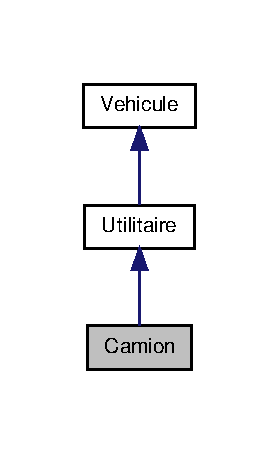
\includegraphics[width=134pt]{class_camion__inherit__graph}
\end{center}
\end{figure}


Graphe de collaboration de Camion:
\nopagebreak
\begin{figure}[H]
\begin{center}
\leavevmode
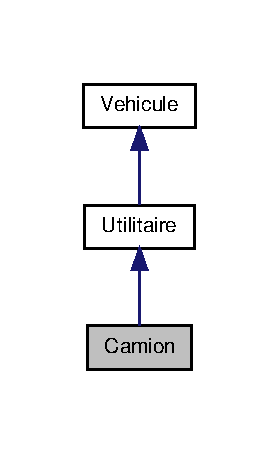
\includegraphics[width=134pt]{class_camion__coll__graph}
\end{center}
\end{figure}
\subsection*{Fonctions membres publiques}
\begin{DoxyCompactItemize}
\item 
\hyperlink{class_camion_ac33dc959ae263b822638aa73b9438ab1}{Camion} (float poids, float volume, string immat, string marque, string modele)
\begin{DoxyCompactList}\small\item\em Constructeur. \item\end{DoxyCompactList}\item 
\hyperlink{class_camion_a5eb698c16331e4fab2ba2cbfebbea8a4}{Camion} ()
\begin{DoxyCompactList}\small\item\em Constructeur. \item\end{DoxyCompactList}\item 
virtual \hyperlink{class_camion_abd045aad98d33e8e353dcf1a6a7832c7}{$\sim$Camion} ()
\begin{DoxyCompactList}\small\item\em Destructeur. \item\end{DoxyCompactList}\item 
float \hyperlink{class_camion_a5eb44123d320dec356d4d335a60b7f28}{getPoidsUtile} ()
\begin{DoxyCompactList}\small\item\em Récupérer poids utile. \item\end{DoxyCompactList}\item 
void \hyperlink{class_camion_a3fe83aa0652ec440e915d983ac46f7d7}{setPoidsUtile} (float poids)
\begin{DoxyCompactList}\small\item\em Modifier poids utile. \item\end{DoxyCompactList}\item 
virtual void \hyperlink{class_camion_a1b7d9e844a03b1a1e7143a7618911157}{afficher} ()
\begin{DoxyCompactList}\small\item\em Afficher utilitaire. \item\end{DoxyCompactList}\item 
virtual void \hyperlink{class_camion_a2c715c85952a7e0bb2948494d79157b8}{save} (fstream \&fs)
\begin{DoxyCompactList}\small\item\em sauvegarder camion \item\end{DoxyCompactList}\end{DoxyCompactItemize}


\subsection{Documentation des constructeurs et destructeur}
\hypertarget{class_camion_ac33dc959ae263b822638aa73b9438ab1}{
\index{Camion@{Camion}!Camion@{Camion}}
\index{Camion@{Camion}!Camion@{Camion}}
\subsubsection[{Camion}]{\setlength{\rightskip}{0pt plus 5cm}Camion::Camion (
\begin{DoxyParamCaption}
\item[{float}]{poids, }
\item[{float}]{volume, }
\item[{string}]{immat, }
\item[{string}]{marque, }
\item[{string}]{modele}
\end{DoxyParamCaption}
)}}
\label{class_camion_ac33dc959ae263b822638aa73b9438ab1}


Constructeur. 

Constructeur de la classe \hyperlink{class_camion}{Camion}


\begin{DoxyParams}[1]{Paramètres}
\mbox{\tt in}  & {\em poids} & réel, poids utile \\
\hline
\mbox{\tt in}  & {\em volume} & réel, volume utile \\
\hline
\mbox{\tt in}  & {\em immat} & chaîne de caractères, le modèle du véhicule \\
\hline
\mbox{\tt in}  & {\em marque} & chaîne de caractères, la marque du véhicule \\
\hline
\mbox{\tt in}  & {\em modele} & chaîne de caractères, le kilométrage du véhicule \\
\hline
\end{DoxyParams}
\hypertarget{class_camion_a5eb698c16331e4fab2ba2cbfebbea8a4}{
\index{Camion@{Camion}!Camion@{Camion}}
\index{Camion@{Camion}!Camion@{Camion}}
\subsubsection[{Camion}]{\setlength{\rightskip}{0pt plus 5cm}Camion::Camion (
\begin{DoxyParamCaption}
{}
\end{DoxyParamCaption}
)}}
\label{class_camion_a5eb698c16331e4fab2ba2cbfebbea8a4}


Constructeur. 

Constructeur par défaut de la classe \hyperlink{class_camion}{Camion} \hypertarget{class_camion_abd045aad98d33e8e353dcf1a6a7832c7}{
\index{Camion@{Camion}!$\sim$Camion@{$\sim$Camion}}
\index{$\sim$Camion@{$\sim$Camion}!Camion@{Camion}}
\subsubsection[{$\sim$Camion}]{\setlength{\rightskip}{0pt plus 5cm}virtual Camion::$\sim$Camion (
\begin{DoxyParamCaption}
{}
\end{DoxyParamCaption}
)\hspace{0.3cm}{\ttfamily  \mbox{[}virtual\mbox{]}}}}
\label{class_camion_abd045aad98d33e8e353dcf1a6a7832c7}


Destructeur. 

Destructeur de la classe \hyperlink{class_camion}{Camion} 

\subsection{Documentation des fonctions membres}
\hypertarget{class_camion_a1b7d9e844a03b1a1e7143a7618911157}{
\index{Camion@{Camion}!afficher@{afficher}}
\index{afficher@{afficher}!Camion@{Camion}}
\subsubsection[{afficher}]{\setlength{\rightskip}{0pt plus 5cm}virtual void Camion::afficher (
\begin{DoxyParamCaption}
{}
\end{DoxyParamCaption}
)\hspace{0.3cm}{\ttfamily  \mbox{[}virtual\mbox{]}}}}
\label{class_camion_a1b7d9e844a03b1a1e7143a7618911157}


Afficher utilitaire. 

Affiche l'utilitaire


\begin{DoxyParams}{Paramètres}
{\em aucun} & \\
\hline
\end{DoxyParams}
\begin{DoxyReturn}{Renvoie}
void 
\end{DoxyReturn}


Réimplémentée à partir de \hyperlink{class_utilitaire_a1092986e687a5a907bc86d252a8416c9}{Utilitaire}.

\hypertarget{class_camion_a5eb44123d320dec356d4d335a60b7f28}{
\index{Camion@{Camion}!getPoidsUtile@{getPoidsUtile}}
\index{getPoidsUtile@{getPoidsUtile}!Camion@{Camion}}
\subsubsection[{getPoidsUtile}]{\setlength{\rightskip}{0pt plus 5cm}float Camion::getPoidsUtile (
\begin{DoxyParamCaption}
{}
\end{DoxyParamCaption}
)}}
\label{class_camion_a5eb44123d320dec356d4d335a60b7f28}


Récupérer poids utile. 

Renvoie le poidsutile


\begin{DoxyParams}{Paramètres}
{\em none} & \\
\hline
\end{DoxyParams}
\begin{DoxyReturn}{Renvoie}
float le poids utile 
\end{DoxyReturn}
\hypertarget{class_camion_a2c715c85952a7e0bb2948494d79157b8}{
\index{Camion@{Camion}!save@{save}}
\index{save@{save}!Camion@{Camion}}
\subsubsection[{save}]{\setlength{\rightskip}{0pt plus 5cm}virtual void Camion::save (
\begin{DoxyParamCaption}
\item[{fstream \&}]{fs}
\end{DoxyParamCaption}
)\hspace{0.3cm}{\ttfamily  \mbox{[}virtual\mbox{]}}}}
\label{class_camion_a2c715c85952a7e0bb2948494d79157b8}


sauvegarder camion 

Sauvegarde le camion


\begin{DoxyParams}[1]{Paramètres}
\mbox{\tt in,out}  & {\em fs} & fstream, le fichier de sauvegarde \\
\hline
\end{DoxyParams}
\begin{DoxyReturn}{Renvoie}
void 
\end{DoxyReturn}


Réimplémentée à partir de \hyperlink{class_utilitaire_a7ee59be5d77191b06b2c959bdf2297b7}{Utilitaire}.

\hypertarget{class_camion_a3fe83aa0652ec440e915d983ac46f7d7}{
\index{Camion@{Camion}!setPoidsUtile@{setPoidsUtile}}
\index{setPoidsUtile@{setPoidsUtile}!Camion@{Camion}}
\subsubsection[{setPoidsUtile}]{\setlength{\rightskip}{0pt plus 5cm}void Camion::setPoidsUtile (
\begin{DoxyParamCaption}
\item[{float}]{poids}
\end{DoxyParamCaption}
)}}
\label{class_camion_a3fe83aa0652ec440e915d983ac46f7d7}


Modifier poids utile. 

Modifie le poids utile


\begin{DoxyParams}[1]{Paramètres}
\mbox{\tt in}  & {\em poids} & réel, le volume utile \\
\hline
\end{DoxyParams}
\begin{DoxyReturn}{Renvoie}
void 
\end{DoxyReturn}


La documentation de cette classe a été générée à partir du fichier suivant :\begin{DoxyCompactItemize}
\item 
inc/\hyperlink{_camion_8h}{Camion.h}\end{DoxyCompactItemize}

\hypertarget{class_c_date}{
\section{Référence de la classe CDate}
\label{class_c_date}\index{CDate@{CDate}}
}


Création et gestion de dates.  




{\ttfamily \#include $<$CDate.h$>$}

\subsection*{Fonctions membres publiques}
\begin{DoxyCompactItemize}
\item 
\hyperlink{class_c_date_abaab9d809338418c9a749ce479fcea61}{CDate} ()
\begin{DoxyCompactList}\small\item\em Constructeur. \item\end{DoxyCompactList}\item 
\hyperlink{class_c_date_ad4cd3f57aa3dd701ffb1e57753f73a6a}{CDate} (const \hyperlink{class_c_date}{CDate} \&date)
\begin{DoxyCompactList}\small\item\em Constructeur. \item\end{DoxyCompactList}\item 
\hyperlink{class_c_date_a674c65d8051308ba639825a012f20eb9}{CDate} (int jour, int mois, int annee)
\begin{DoxyCompactList}\small\item\em Constructeur. \item\end{DoxyCompactList}\item 
\hyperlink{class_c_date_a27cb391423bff726cd1a9b1bed10eea9}{$\sim$CDate} ()
\begin{DoxyCompactList}\small\item\em Destructeur. \item\end{DoxyCompactList}\item 
int \hyperlink{class_c_date_a1b2130af68061448ba2f2eff741570ac}{getJour} ()
\begin{DoxyCompactList}\small\item\em Accéder au jour. \item\end{DoxyCompactList}\item 
int \hyperlink{class_c_date_a499fa44735a061481ed6d47e3382fa6a}{getMois} ()
\begin{DoxyCompactList}\small\item\em Accéder au mois. \item\end{DoxyCompactList}\item 
int \hyperlink{class_c_date_af37b56e430b856c1b2360cfc7c284bf0}{getAnnee} ()
\begin{DoxyCompactList}\small\item\em Accéder à l'année. \item\end{DoxyCompactList}\item 
void \hyperlink{class_c_date_a9ba9c1985bd904ae24b8d10d580c9dfa}{setJour} (int jour)
\begin{DoxyCompactList}\small\item\em Modifier jour. \item\end{DoxyCompactList}\item 
void \hyperlink{class_c_date_a1d8d023913f19ee53edb9857b5cec7e5}{setMois} (int mois)
\begin{DoxyCompactList}\small\item\em Modifier mois. \item\end{DoxyCompactList}\item 
void \hyperlink{class_c_date_a3340b3febf97ddad564a26784cd739da}{setAnnee} (int annee)
\begin{DoxyCompactList}\small\item\em Modifier année. \item\end{DoxyCompactList}\item 
string \hyperlink{class_c_date_a4182c878d46bd44c8a78c82cccc504da}{GetStrMois} ()
\begin{DoxyCompactList}\small\item\em Accès à l'intitulé du mois. \item\end{DoxyCompactList}\item 
int \hyperlink{class_c_date_a04a7801cc2f9441321735bf41602d3b2}{nbJours} (int mois, int annee)
\begin{DoxyCompactList}\small\item\em Indique le nombre de jours du mois. \item\end{DoxyCompactList}\item 
bool \hyperlink{class_c_date_a02dad71347f444a5ee5a889f62fb5f4e}{estBissextile} (int annee)
\begin{DoxyCompactList}\small\item\em Indique si une année est bissextile. \item\end{DoxyCompactList}\item 
bool \hyperlink{class_c_date_a45a71c91bd790e7b84405c8128e4094b}{validerDate} (int jour, int mois, int annee)
\begin{DoxyCompactList}\small\item\em Permet de valider une date. \item\end{DoxyCompactList}\item 
bool \hyperlink{class_c_date_a82e5b049e86145b62893f194b5638ad6}{operator==} (const \hyperlink{class_c_date}{CDate} \&date) const 
\begin{DoxyCompactList}\small\item\em Égalité dates. \item\end{DoxyCompactList}\item 
bool \hyperlink{class_c_date_a2764c65e43a4ee956cd16f8ce242dbc7}{operator$<$} (const \hyperlink{class_c_date}{CDate} \&date) const 
\begin{DoxyCompactList}\small\item\em Infériorité dates. \item\end{DoxyCompactList}\item 
bool \hyperlink{class_c_date_ac653ba135b3681a64448872b2d6a0c17}{operator$>$} (const \hyperlink{class_c_date}{CDate} \&date) const 
\begin{DoxyCompactList}\small\item\em Supériorité dates. \item\end{DoxyCompactList}\item 
void \hyperlink{class_c_date_a9b58a7c96cf53352328906e30891e4e4}{afficher} ()
\begin{DoxyCompactList}\small\item\em Afficher date. \item\end{DoxyCompactList}\end{DoxyCompactItemize}
\subsection*{Fonctions membres publiques statiques}
\begin{DoxyCompactItemize}
\item 
static \hyperlink{class_c_date}{CDate} \hyperlink{class_c_date_a5367206ed910298afbf1bf57efe47c92}{today} ()
\begin{DoxyCompactList}\small\item\em Date du jour. \item\end{DoxyCompactList}\end{DoxyCompactItemize}


\subsection{Description détaillée}
Création et gestion de dates. Cette classe propose des outils pour gérer une date 

\subsection{Documentation des constructeurs et destructeur}
\hypertarget{class_c_date_abaab9d809338418c9a749ce479fcea61}{
\index{CDate@{CDate}!CDate@{CDate}}
\index{CDate@{CDate}!CDate@{CDate}}
\subsubsection[{CDate}]{\setlength{\rightskip}{0pt plus 5cm}CDate::CDate (
\begin{DoxyParamCaption}
{}
\end{DoxyParamCaption}
)}}
\label{class_c_date_abaab9d809338418c9a749ce479fcea61}


Constructeur. 

Constructeur par défaut de la classe date


\begin{DoxyParams}{Paramètres}
{\em aucun} & \\
\hline
\end{DoxyParams}
\hypertarget{class_c_date_ad4cd3f57aa3dd701ffb1e57753f73a6a}{
\index{CDate@{CDate}!CDate@{CDate}}
\index{CDate@{CDate}!CDate@{CDate}}
\subsubsection[{CDate}]{\setlength{\rightskip}{0pt plus 5cm}CDate::CDate (
\begin{DoxyParamCaption}
\item[{const {\bf CDate} \&}]{date}
\end{DoxyParamCaption}
)}}
\label{class_c_date_ad4cd3f57aa3dd701ffb1e57753f73a6a}


Constructeur. 

Constructeur par copie de la classe date


\begin{DoxyParams}[1]{Paramètres}
\mbox{\tt in}  & {\em date} & \hyperlink{class_c_date}{CDate}, une date \\
\hline
\end{DoxyParams}
\hypertarget{class_c_date_a674c65d8051308ba639825a012f20eb9}{
\index{CDate@{CDate}!CDate@{CDate}}
\index{CDate@{CDate}!CDate@{CDate}}
\subsubsection[{CDate}]{\setlength{\rightskip}{0pt plus 5cm}CDate::CDate (
\begin{DoxyParamCaption}
\item[{int}]{jour, }
\item[{int}]{mois, }
\item[{int}]{annee}
\end{DoxyParamCaption}
)}}
\label{class_c_date_a674c65d8051308ba639825a012f20eb9}


Constructeur. 

Constructeur de la classe date


\begin{DoxyParams}[1]{Paramètres}
\mbox{\tt in}  & {\em jour} & entier, le jour \\
\hline
\mbox{\tt in}  & {\em mois} & entier, le mois \\
\hline
\mbox{\tt in}  & {\em annee} & entier, l'année \\
\hline
\end{DoxyParams}
\hypertarget{class_c_date_a27cb391423bff726cd1a9b1bed10eea9}{
\index{CDate@{CDate}!$\sim$CDate@{$\sim$CDate}}
\index{$\sim$CDate@{$\sim$CDate}!CDate@{CDate}}
\subsubsection[{$\sim$CDate}]{\setlength{\rightskip}{0pt plus 5cm}CDate::$\sim$CDate (
\begin{DoxyParamCaption}
{}
\end{DoxyParamCaption}
)}}
\label{class_c_date_a27cb391423bff726cd1a9b1bed10eea9}


Destructeur. 

Destructeur de la classe date


\begin{DoxyParams}{Paramètres}
{\em aucun} & \\
\hline
\end{DoxyParams}


\subsection{Documentation des fonctions membres}
\hypertarget{class_c_date_a9b58a7c96cf53352328906e30891e4e4}{
\index{CDate@{CDate}!afficher@{afficher}}
\index{afficher@{afficher}!CDate@{CDate}}
\subsubsection[{afficher}]{\setlength{\rightskip}{0pt plus 5cm}void CDate::afficher (
\begin{DoxyParamCaption}
{}
\end{DoxyParamCaption}
)}}
\label{class_c_date_a9b58a7c96cf53352328906e30891e4e4}


Afficher date. 

Affiche la date


\begin{DoxyParams}{Paramètres}
{\em aucun} & \\
\hline
\end{DoxyParams}
\begin{DoxyReturn}{Renvoie}
void 
\end{DoxyReturn}
\hypertarget{class_c_date_a02dad71347f444a5ee5a889f62fb5f4e}{
\index{CDate@{CDate}!estBissextile@{estBissextile}}
\index{estBissextile@{estBissextile}!CDate@{CDate}}
\subsubsection[{estBissextile}]{\setlength{\rightskip}{0pt plus 5cm}bool CDate::estBissextile (
\begin{DoxyParamCaption}
\item[{int}]{annee}
\end{DoxyParamCaption}
)}}
\label{class_c_date_a02dad71347f444a5ee5a889f62fb5f4e}


Indique si une année est bissextile. 

Permet de connaitre si une année est bissextile ou pas


\begin{DoxyParams}[1]{Paramètres}
\mbox{\tt in}  & {\em annee} & entier, l'année \\
\hline
\end{DoxyParams}
\begin{DoxyReturn}{Renvoie}
bool, vrai si l'année est bissextile 

bool, faux si l'année n'est pas bissextile 
\end{DoxyReturn}
\hypertarget{class_c_date_af37b56e430b856c1b2360cfc7c284bf0}{
\index{CDate@{CDate}!getAnnee@{getAnnee}}
\index{getAnnee@{getAnnee}!CDate@{CDate}}
\subsubsection[{getAnnee}]{\setlength{\rightskip}{0pt plus 5cm}int CDate::getAnnee (
\begin{DoxyParamCaption}
{}
\end{DoxyParamCaption}
)\hspace{0.3cm}{\ttfamily  \mbox{[}inline\mbox{]}}}}
\label{class_c_date_af37b56e430b856c1b2360cfc7c284bf0}


Accéder à l'année. 

Permet d'obtenir l'année de la date


\begin{DoxyParams}{Paramètres}
{\em aucun} & \\
\hline
\end{DoxyParams}
\begin{DoxyReturn}{Renvoie}
un entier, l'année de la date 
\end{DoxyReturn}
\hypertarget{class_c_date_a1b2130af68061448ba2f2eff741570ac}{
\index{CDate@{CDate}!getJour@{getJour}}
\index{getJour@{getJour}!CDate@{CDate}}
\subsubsection[{getJour}]{\setlength{\rightskip}{0pt plus 5cm}int CDate::getJour (
\begin{DoxyParamCaption}
{}
\end{DoxyParamCaption}
)\hspace{0.3cm}{\ttfamily  \mbox{[}inline\mbox{]}}}}
\label{class_c_date_a1b2130af68061448ba2f2eff741570ac}


Accéder au jour. 

Permet d'obtenir le jour de la date


\begin{DoxyParams}{Paramètres}
{\em aucun} & \\
\hline
\end{DoxyParams}
\begin{DoxyReturn}{Renvoie}
un entier, le jour de la date 
\end{DoxyReturn}
\hypertarget{class_c_date_a499fa44735a061481ed6d47e3382fa6a}{
\index{CDate@{CDate}!getMois@{getMois}}
\index{getMois@{getMois}!CDate@{CDate}}
\subsubsection[{getMois}]{\setlength{\rightskip}{0pt plus 5cm}int CDate::getMois (
\begin{DoxyParamCaption}
{}
\end{DoxyParamCaption}
)\hspace{0.3cm}{\ttfamily  \mbox{[}inline\mbox{]}}}}
\label{class_c_date_a499fa44735a061481ed6d47e3382fa6a}


Accéder au mois. 

Permet d'obtenir le mois de la date


\begin{DoxyParams}{Paramètres}
{\em aucun} & \\
\hline
\end{DoxyParams}
\begin{DoxyReturn}{Renvoie}
un entier, le mois de la date 
\end{DoxyReturn}
\hypertarget{class_c_date_a4182c878d46bd44c8a78c82cccc504da}{
\index{CDate@{CDate}!GetStrMois@{GetStrMois}}
\index{GetStrMois@{GetStrMois}!CDate@{CDate}}
\subsubsection[{GetStrMois}]{\setlength{\rightskip}{0pt plus 5cm}string CDate::GetStrMois (
\begin{DoxyParamCaption}
{}
\end{DoxyParamCaption}
)}}
\label{class_c_date_a4182c878d46bd44c8a78c82cccc504da}


Accès à l'intitulé du mois. 

Permet de récupérer le nom du mois


\begin{DoxyParams}{Paramètres}
{\em aucun} & \\
\hline
\end{DoxyParams}
\begin{DoxyReturn}{Renvoie}
chaine de caractères, le nom du mois 
\end{DoxyReturn}
\hypertarget{class_c_date_a04a7801cc2f9441321735bf41602d3b2}{
\index{CDate@{CDate}!nbJours@{nbJours}}
\index{nbJours@{nbJours}!CDate@{CDate}}
\subsubsection[{nbJours}]{\setlength{\rightskip}{0pt plus 5cm}int CDate::nbJours (
\begin{DoxyParamCaption}
\item[{int}]{mois, }
\item[{int}]{annee}
\end{DoxyParamCaption}
)}}
\label{class_c_date_a04a7801cc2f9441321735bf41602d3b2}


Indique le nombre de jours du mois. 

Permet de connaitre le nombre de jours d'un mois par rapport à l'année. Appel de la fonction estBissextile


\begin{DoxyParams}[1]{Paramètres}
\mbox{\tt in}  & {\em mois} & entier, le mois \\
\hline
\mbox{\tt in}  & {\em annee} & entier, l'année \\
\hline
\end{DoxyParams}
\begin{DoxyReturn}{Renvoie}
un entier, le nombre de jours du mois 
\end{DoxyReturn}
\hypertarget{class_c_date_a2764c65e43a4ee956cd16f8ce242dbc7}{
\index{CDate@{CDate}!operator$<$@{operator$<$}}
\index{operator$<$@{operator$<$}!CDate@{CDate}}
\subsubsection[{operator$<$}]{\setlength{\rightskip}{0pt plus 5cm}bool CDate::operator$<$ (
\begin{DoxyParamCaption}
\item[{const {\bf CDate} \&}]{date}
\end{DoxyParamCaption}
) const}}
\label{class_c_date_a2764c65e43a4ee956cd16f8ce242dbc7}


Infériorité dates. 

Renvoie vrai si la date passée en paramètre est inférieure


\begin{DoxyParams}[1]{Paramètres}
\mbox{\tt in}  & {\em date} & Date, la date à comparer \\
\hline
\end{DoxyParams}
\begin{DoxyReturn}{Renvoie}
bool, vrai si la date passée en paramètre est inférieure 

bool, faux si la date passée en paramètre n'est pas inférieure 
\end{DoxyReturn}
\hypertarget{class_c_date_a82e5b049e86145b62893f194b5638ad6}{
\index{CDate@{CDate}!operator==@{operator==}}
\index{operator==@{operator==}!CDate@{CDate}}
\subsubsection[{operator==}]{\setlength{\rightskip}{0pt plus 5cm}bool CDate::operator== (
\begin{DoxyParamCaption}
\item[{const {\bf CDate} \&}]{date}
\end{DoxyParamCaption}
) const}}
\label{class_c_date_a82e5b049e86145b62893f194b5638ad6}


Égalité dates. 

Renvoie vrai si deux dates sont égales, faux sinon


\begin{DoxyParams}[1]{Paramètres}
\mbox{\tt in}  & {\em date} & Date, la date à comparer \\
\hline
\end{DoxyParams}
\begin{DoxyReturn}{Renvoie}
bool, vrai si les deux dates sont égales 

bool, faux si les deux dates sont différentes 
\end{DoxyReturn}
\hypertarget{class_c_date_ac653ba135b3681a64448872b2d6a0c17}{
\index{CDate@{CDate}!operator$>$@{operator$>$}}
\index{operator$>$@{operator$>$}!CDate@{CDate}}
\subsubsection[{operator$>$}]{\setlength{\rightskip}{0pt plus 5cm}bool CDate::operator$>$ (
\begin{DoxyParamCaption}
\item[{const {\bf CDate} \&}]{date}
\end{DoxyParamCaption}
) const}}
\label{class_c_date_ac653ba135b3681a64448872b2d6a0c17}


Supériorité dates. 

Renvoie vrai si la date passée en paramètre est supérieure


\begin{DoxyParams}[1]{Paramètres}
\mbox{\tt in}  & {\em date} & Date, la date à comparer \\
\hline
\end{DoxyParams}
\begin{DoxyReturn}{Renvoie}
bool, vrai si la date passée en paramètre est supérieure 

bool, faux si la date passée en paramètre n'est pas supérieure 
\end{DoxyReturn}
\hypertarget{class_c_date_a3340b3febf97ddad564a26784cd739da}{
\index{CDate@{CDate}!setAnnee@{setAnnee}}
\index{setAnnee@{setAnnee}!CDate@{CDate}}
\subsubsection[{setAnnee}]{\setlength{\rightskip}{0pt plus 5cm}void CDate::setAnnee (
\begin{DoxyParamCaption}
\item[{int}]{annee}
\end{DoxyParamCaption}
)\hspace{0.3cm}{\ttfamily  \mbox{[}inline\mbox{]}}}}
\label{class_c_date_a3340b3febf97ddad564a26784cd739da}


Modifier année. 

Permet de modifier l'année de la date


\begin{DoxyParams}[1]{Paramètres}
\mbox{\tt in}  & {\em annee} & entier, la nouvelle année \\
\hline
\end{DoxyParams}
\begin{DoxyReturn}{Renvoie}
void 
\end{DoxyReturn}
\hypertarget{class_c_date_a9ba9c1985bd904ae24b8d10d580c9dfa}{
\index{CDate@{CDate}!setJour@{setJour}}
\index{setJour@{setJour}!CDate@{CDate}}
\subsubsection[{setJour}]{\setlength{\rightskip}{0pt plus 5cm}void CDate::setJour (
\begin{DoxyParamCaption}
\item[{int}]{jour}
\end{DoxyParamCaption}
)\hspace{0.3cm}{\ttfamily  \mbox{[}inline\mbox{]}}}}
\label{class_c_date_a9ba9c1985bd904ae24b8d10d580c9dfa}


Modifier jour. 

Permet de modifier le jour de la date


\begin{DoxyParams}[1]{Paramètres}
\mbox{\tt in}  & {\em jour} & entier, le nouveau jour \\
\hline
\end{DoxyParams}
\begin{DoxyReturn}{Renvoie}
void 
\end{DoxyReturn}
\hypertarget{class_c_date_a1d8d023913f19ee53edb9857b5cec7e5}{
\index{CDate@{CDate}!setMois@{setMois}}
\index{setMois@{setMois}!CDate@{CDate}}
\subsubsection[{setMois}]{\setlength{\rightskip}{0pt plus 5cm}void CDate::setMois (
\begin{DoxyParamCaption}
\item[{int}]{mois}
\end{DoxyParamCaption}
)\hspace{0.3cm}{\ttfamily  \mbox{[}inline\mbox{]}}}}
\label{class_c_date_a1d8d023913f19ee53edb9857b5cec7e5}


Modifier mois. 

Permet de modifier le mois de la date


\begin{DoxyParams}[1]{Paramètres}
\mbox{\tt in}  & {\em mois} & entier, le nouveau mois \\
\hline
\end{DoxyParams}
\begin{DoxyReturn}{Renvoie}
void 
\end{DoxyReturn}
\hypertarget{class_c_date_a5367206ed910298afbf1bf57efe47c92}{
\index{CDate@{CDate}!today@{today}}
\index{today@{today}!CDate@{CDate}}
\subsubsection[{today}]{\setlength{\rightskip}{0pt plus 5cm}static {\bf CDate} CDate::today (
\begin{DoxyParamCaption}
{}
\end{DoxyParamCaption}
)\hspace{0.3cm}{\ttfamily  \mbox{[}static\mbox{]}}}}
\label{class_c_date_a5367206ed910298afbf1bf57efe47c92}


Date du jour. 

Renvoie la date du jour


\begin{DoxyParams}{Paramètres}
{\em aucun} & \\
\hline
\end{DoxyParams}
\begin{DoxyReturn}{Renvoie}
\hyperlink{class_c_date}{CDate}, la date du jour 
\end{DoxyReturn}
\hypertarget{class_c_date_a45a71c91bd790e7b84405c8128e4094b}{
\index{CDate@{CDate}!validerDate@{validerDate}}
\index{validerDate@{validerDate}!CDate@{CDate}}
\subsubsection[{validerDate}]{\setlength{\rightskip}{0pt plus 5cm}bool CDate::validerDate (
\begin{DoxyParamCaption}
\item[{int}]{jour, }
\item[{int}]{mois, }
\item[{int}]{annee}
\end{DoxyParamCaption}
)}}
\label{class_c_date_a45a71c91bd790e7b84405c8128e4094b}


Permet de valider une date. 

Vérifie si une année est valide ou pas


\begin{DoxyParams}[1]{Paramètres}
\mbox{\tt in}  & {\em jour} & entier, le jour \\
\hline
\mbox{\tt in}  & {\em mois} & entier, le mois \\
\hline
\mbox{\tt in}  & {\em annee} & entier, l'année \\
\hline
\end{DoxyParams}
\begin{DoxyReturn}{Renvoie}
bool, vrai si la date est valide 

bool, faux si la date n'est pas valide 
\end{DoxyReturn}


La documentation de cette classe a été générée à partir du fichier suivant :\begin{DoxyCompactItemize}
\item 
inc/\hyperlink{_c_date_8h}{CDate.h}\end{DoxyCompactItemize}

\hypertarget{classerreur}{
\section{Référence de la classe erreur}
\label{classerreur}\index{erreur@{erreur}}
}
\subsection*{Fonctions membres publiques}
\begin{DoxyCompactItemize}
\item 
\hypertarget{classerreur_a95060559d107fe1a250fb1fb0f9f0cfa}{
{\bfseries erreur} (int c)}
\label{classerreur_a95060559d107fe1a250fb1fb0f9f0cfa}

\item 
\hypertarget{classerreur_af51ada62a9c20d282865f4fb8d3fdeda}{
{\bfseries erreur} (const \hyperlink{classerreur}{erreur} \&source)}
\label{classerreur_af51ada62a9c20d282865f4fb8d3fdeda}

\end{DoxyCompactItemize}
\subsection*{Attributs publics}
\begin{DoxyCompactItemize}
\item 
\hypertarget{classerreur_a32cfb866208f19b7291269e3b53180ad}{
int {\bfseries cause}}
\label{classerreur_a32cfb866208f19b7291269e3b53180ad}

\end{DoxyCompactItemize}


La documentation de cette classe a été générée à partir du fichier suivant :\begin{DoxyCompactItemize}
\item 
inc/Erreur.h\end{DoxyCompactItemize}

\hypertarget{class_liste_reservations}{
\section{Référence de la classe ListeReservations}
\label{class_liste_reservations}\index{ListeReservations@{ListeReservations}}
}
\subsection*{Fonctions membres publiques}
\begin{DoxyCompactItemize}
\item 
\hyperlink{class_liste_reservations_a588814a2a1a844ad70e790d1cf7f3d45}{ListeReservations} (fstream \&inFile)
\begin{DoxyCompactList}\small\item\em Constructeur. \item\end{DoxyCompactList}\item 
\hyperlink{class_liste_reservations_a32f73522c4b7e1dc98dc6ed8a06e7ec6}{$\sim$ListeReservations} ()
\begin{DoxyCompactList}\small\item\em Destructeur. \item\end{DoxyCompactList}\item 
bool \hyperlink{class_liste_reservations_abc616def701c55e0643f7ace4e0dd0c5}{ajouterReservation} (\hyperlink{class_reservation}{Reservation} res)
\begin{DoxyCompactList}\small\item\em Ajouter réservation. \item\end{DoxyCompactList}\item 
void \hyperlink{class_liste_reservations_a6a199865ea417f472c46cd981bdb9e2c}{afficher} (\hyperlink{class_parc}{Parc} p)
\begin{DoxyCompactList}\small\item\em Afficher liste complète. \item\end{DoxyCompactList}\item 
void \hyperlink{class_liste_reservations_a0d55928f73787fe75e77df3fd79da52e}{sauvegarder} (string nomFichier)
\begin{DoxyCompactList}\small\item\em Sauvegarder liste réservations. \item\end{DoxyCompactList}\end{DoxyCompactItemize}


\subsection{Documentation des constructeurs et destructeur}
\hypertarget{class_liste_reservations_a588814a2a1a844ad70e790d1cf7f3d45}{
\index{ListeReservations@{ListeReservations}!ListeReservations@{ListeReservations}}
\index{ListeReservations@{ListeReservations}!ListeReservations@{ListeReservations}}
\subsubsection[{ListeReservations}]{\setlength{\rightskip}{0pt plus 5cm}ListeReservations::ListeReservations (
\begin{DoxyParamCaption}
\item[{fstream \&}]{inFile}
\end{DoxyParamCaption}
)}}
\label{class_liste_reservations_a588814a2a1a844ad70e790d1cf7f3d45}


Constructeur. 

Constructeur de la classe \hyperlink{class_liste_reservations}{ListeReservations}


\begin{DoxyParams}[1]{Paramètres}
\mbox{\tt in,out}  & {\em inFile} & fstream, le fichier contenant la liste des réservations \\
\hline
\end{DoxyParams}
\hypertarget{class_liste_reservations_a32f73522c4b7e1dc98dc6ed8a06e7ec6}{
\index{ListeReservations@{ListeReservations}!$\sim$ListeReservations@{$\sim$ListeReservations}}
\index{$\sim$ListeReservations@{$\sim$ListeReservations}!ListeReservations@{ListeReservations}}
\subsubsection[{$\sim$ListeReservations}]{\setlength{\rightskip}{0pt plus 5cm}ListeReservations::$\sim$ListeReservations (
\begin{DoxyParamCaption}
{}
\end{DoxyParamCaption}
)}}
\label{class_liste_reservations_a32f73522c4b7e1dc98dc6ed8a06e7ec6}


Destructeur. 

Destructeur de la classe \hyperlink{class_liste_reservations}{ListeReservations}


\begin{DoxyParams}{Paramètres}
{\em aucun} & \\
\hline
\end{DoxyParams}


\subsection{Documentation des fonctions membres}
\hypertarget{class_liste_reservations_a6a199865ea417f472c46cd981bdb9e2c}{
\index{ListeReservations@{ListeReservations}!afficher@{afficher}}
\index{afficher@{afficher}!ListeReservations@{ListeReservations}}
\subsubsection[{afficher}]{\setlength{\rightskip}{0pt plus 5cm}void ListeReservations::afficher (
\begin{DoxyParamCaption}
\item[{{\bf Parc}}]{p}
\end{DoxyParamCaption}
)}}
\label{class_liste_reservations_a6a199865ea417f472c46cd981bdb9e2c}


Afficher liste complète. 

Affiche la liste des réservations. La liste affichée peut contenir toutes les réservations, les réservations dont la date de départ est égale à date ou les véhicules restituables. Sont considérés restituables tous les véhicules dont la date de retour est celle du jour courant.


\begin{DoxyParams}[1]{Paramètres}
\mbox{\tt in}  & {\em p} & \hyperlink{class_parc}{Parc}, le parc de véhicule dans lequel rechercher les informations sur les véhicules réservés \\
\hline
\end{DoxyParams}
\begin{DoxyReturn}{Renvoie}
void 
\end{DoxyReturn}
\hypertarget{class_liste_reservations_abc616def701c55e0643f7ace4e0dd0c5}{
\index{ListeReservations@{ListeReservations}!ajouterReservation@{ajouterReservation}}
\index{ajouterReservation@{ajouterReservation}!ListeReservations@{ListeReservations}}
\subsubsection[{ajouterReservation}]{\setlength{\rightskip}{0pt plus 5cm}bool ListeReservations::ajouterReservation (
\begin{DoxyParamCaption}
\item[{{\bf Reservation}}]{res}
\end{DoxyParamCaption}
)}}
\label{class_liste_reservations_abc616def701c55e0643f7ace4e0dd0c5}


Ajouter réservation. 

Permet d'ajouter une réservation à la liste


\begin{DoxyParams}[1]{Paramètres}
\mbox{\tt in}  & {\em res} & \hyperlink{class_reservation}{Reservation}, la réservation à ajouter \\
\hline
\end{DoxyParams}
\begin{DoxyReturn}{Renvoie}
bool vrai si la réservation a été ajoutée à la liste 

bool faux si la réservation n'a pas pu être ajoutée à la liste 
\end{DoxyReturn}
\hypertarget{class_liste_reservations_a0d55928f73787fe75e77df3fd79da52e}{
\index{ListeReservations@{ListeReservations}!sauvegarder@{sauvegarder}}
\index{sauvegarder@{sauvegarder}!ListeReservations@{ListeReservations}}
\subsubsection[{sauvegarder}]{\setlength{\rightskip}{0pt plus 5cm}void ListeReservations::sauvegarder (
\begin{DoxyParamCaption}
\item[{string}]{nomFichier}
\end{DoxyParamCaption}
)}}
\label{class_liste_reservations_a0d55928f73787fe75e77df3fd79da52e}


Sauvegarder liste réservations. 

Sauvegarde la liste des réservations dans un fichier


\begin{DoxyParams}[1]{Paramètres}
\mbox{\tt in,out}  & {\em nomFichier} & string, le nom du fichier de sauvegarde \\
\hline
\end{DoxyParams}
\begin{DoxyReturn}{Renvoie}
void 
\end{DoxyReturn}


La documentation de cette classe a été générée à partir du fichier suivant :\begin{DoxyCompactItemize}
\item 
inc/\hyperlink{_liste_reservations_8h}{ListeReservations.h}\end{DoxyCompactItemize}

\hypertarget{class_location}{
\section{Référence de la classe Location}
\label{class_location}\index{Location@{Location}}
}


{\ttfamily \#include $<$Location.h$>$}

\subsection*{Fonctions membres publiques}
\begin{DoxyCompactItemize}
\item 
\hyperlink{class_location_a87790c14997fd8cdd12080c78c9794bb}{Location} ()
\begin{DoxyCompactList}\small\item\em Constructeur. \item\end{DoxyCompactList}\item 
\hyperlink{class_location_a5a09ef0b7e8bd346553572e4a17e916a}{Location} (\hyperlink{class_vehicule}{Vehicule} $\ast$vehicule, \hyperlink{class_c_date}{CDate} dateDepart, \hyperlink{class_c_date}{CDate} dateRetourPrevu, \hyperlink{class_c_date}{CDate} dateRetourReel)
\begin{DoxyCompactList}\small\item\em Constructeur. \item\end{DoxyCompactList}\item 
\hyperlink{class_location_af5be2c6550bbd96137cbb3144ec3c529}{$\sim$Location} ()
\begin{DoxyCompactList}\small\item\em Destructeur. \item\end{DoxyCompactList}\item 
\hyperlink{class_vehicule}{Vehicule} $\ast$ \hyperlink{class_location_a3f130f10a4a558d6b792b1e538e9fb40}{getVehicule} ()
\begin{DoxyCompactList}\small\item\em Accéder au véhicule. \item\end{DoxyCompactList}\item 
void \hyperlink{class_location_a66eaf6883a88c65a6281ccf111db3c03}{setVehicule} (\hyperlink{class_vehicule}{Vehicule} $\ast$veh)
\begin{DoxyCompactList}\small\item\em Modifier véhicule. \item\end{DoxyCompactList}\item 
\hyperlink{class_c_date}{CDate} \hyperlink{class_location_a02e6d2fc6aca23b344994df6e128ccff}{getDate} (char type)
\begin{DoxyCompactList}\small\item\em Accéder date début. \item\end{DoxyCompactList}\item 
void \hyperlink{class_location_ab01cd2764d9db2771d2f2c7befa8123c}{setDate} (\hyperlink{class_c_date}{CDate} date, char type)
\begin{DoxyCompactList}\small\item\em Modifier date. \item\end{DoxyCompactList}\item 
void \hyperlink{class_location_ad7dadc3847da51c3c012f0647f011706}{afficher} ()
\begin{DoxyCompactList}\small\item\em Afficher location. \item\end{DoxyCompactList}\end{DoxyCompactItemize}


\subsection{Description détaillée}
Remarques Déclarer un pointeur \{ \hyperlink{class_vehicule}{Vehicule} $\ast$m\_\-vehicule; \} affecter un pointeur \{ \hyperlink{class_vehicule}{Vehicule} veh; m\_\-vehicule =  \} allouer un pointeur \{ m\_\-vehicule = new Vehicule() ; \} 

\subsection{Documentation des constructeurs et destructeur}
\hypertarget{class_location_a87790c14997fd8cdd12080c78c9794bb}{
\index{Location@{Location}!Location@{Location}}
\index{Location@{Location}!Location@{Location}}
\subsubsection[{Location}]{\setlength{\rightskip}{0pt plus 5cm}Location::Location (
\begin{DoxyParamCaption}
{}
\end{DoxyParamCaption}
)}}
\label{class_location_a87790c14997fd8cdd12080c78c9794bb}


Constructeur. 

Constructeur par défaut de la classe \hyperlink{class_location}{Location}


\begin{DoxyParams}{Paramètres}
{\em aucun} & \\
\hline
\end{DoxyParams}
\hypertarget{class_location_a5a09ef0b7e8bd346553572e4a17e916a}{
\index{Location@{Location}!Location@{Location}}
\index{Location@{Location}!Location@{Location}}
\subsubsection[{Location}]{\setlength{\rightskip}{0pt plus 5cm}Location::Location (
\begin{DoxyParamCaption}
\item[{{\bf Vehicule} $\ast$}]{vehicule, }
\item[{{\bf CDate}}]{dateDepart, }
\item[{{\bf CDate}}]{dateRetourPrevu, }
\item[{{\bf CDate}}]{dateRetourReel}
\end{DoxyParamCaption}
)}}
\label{class_location_a5a09ef0b7e8bd346553572e4a17e916a}


Constructeur. 

Constructeur de la classe \hyperlink{class_location}{Location}


\begin{DoxyParams}{Paramètres}
{\em vehicule,un} & pointeur de véhicule \\
\hline
{\em dateDepart,objet} & \hyperlink{class_c_date}{CDate}, la date de début de location, NULL si le véhicule n'est pas loué \\
\hline
{\em dateRetourPrevue,objet} & \hyperlink{class_c_date}{CDate}, la date de fin prévue de la location, NULL si le véhicule n'est pas loué \\
\hline
{\em dateRetourReel,objet} & \hyperlink{class_c_date}{CDate}, la date réelle du retour location, NULL si le véhicule n'est pas loué ou s'il est en cours de location \\
\hline
\end{DoxyParams}
\hypertarget{class_location_af5be2c6550bbd96137cbb3144ec3c529}{
\index{Location@{Location}!$\sim$Location@{$\sim$Location}}
\index{$\sim$Location@{$\sim$Location}!Location@{Location}}
\subsubsection[{$\sim$Location}]{\setlength{\rightskip}{0pt plus 5cm}Location::$\sim$Location (
\begin{DoxyParamCaption}
{}
\end{DoxyParamCaption}
)}}
\label{class_location_af5be2c6550bbd96137cbb3144ec3c529}


Destructeur. 

Destructeur de la classe \hyperlink{class_location}{Location}


\begin{DoxyParams}{Paramètres}
{\em aucun} & \\
\hline
\end{DoxyParams}


\subsection{Documentation des fonctions membres}
\hypertarget{class_location_ad7dadc3847da51c3c012f0647f011706}{
\index{Location@{Location}!afficher@{afficher}}
\index{afficher@{afficher}!Location@{Location}}
\subsubsection[{afficher}]{\setlength{\rightskip}{0pt plus 5cm}void Location::afficher (
\begin{DoxyParamCaption}
{}
\end{DoxyParamCaption}
)}}
\label{class_location_ad7dadc3847da51c3c012f0647f011706}


Afficher location. 

Affiche la location


\begin{DoxyParams}{Paramètres}
{\em aucun} & \\
\hline
\end{DoxyParams}
\begin{DoxyReturn}{Renvoie}
void 
\end{DoxyReturn}
\hypertarget{class_location_a02e6d2fc6aca23b344994df6e128ccff}{
\index{Location@{Location}!getDate@{getDate}}
\index{getDate@{getDate}!Location@{Location}}
\subsubsection[{getDate}]{\setlength{\rightskip}{0pt plus 5cm}{\bf CDate} Location::getDate (
\begin{DoxyParamCaption}
\item[{char}]{type}
\end{DoxyParamCaption}
)}}
\label{class_location_a02e6d2fc6aca23b344994df6e128ccff}


Accéder date début. 

Permet d'obtenir les dates associées à la location : date de départ, date de retour prévu, date de retour réel


\begin{DoxyParams}{Paramètres}
{\em type,caractère,le} & type de date souhaité : d pour dateDepart, r pour dateRetourReel, p pour dateRetourPrevu \\
\hline
\end{DoxyParams}
\begin{DoxyReturn}{Renvoie}
un objet \hyperlink{class_c_date}{CDate} 
\end{DoxyReturn}

\begin{DoxyExceptions}{Exceptions}
{\em si} & type différent de \char`\"{}d\char`\"{}, \char`\"{}r\char`\"{}, ou \char`\"{}p\char`\"{}, lance une erreur \char`\"{}erreur(1) mauvais type de date\char`\"{} \\
\hline
\end{DoxyExceptions}
\hypertarget{class_location_a3f130f10a4a558d6b792b1e538e9fb40}{
\index{Location@{Location}!getVehicule@{getVehicule}}
\index{getVehicule@{getVehicule}!Location@{Location}}
\subsubsection[{getVehicule}]{\setlength{\rightskip}{0pt plus 5cm}{\bf Vehicule}$\ast$ Location::getVehicule (
\begin{DoxyParamCaption}
{}
\end{DoxyParamCaption}
)}}
\label{class_location_a3f130f10a4a558d6b792b1e538e9fb40}


Accéder au véhicule. 

Permet d'obtenir le véhicule à partir de son immatriculation


\begin{DoxyParams}{Paramètres}
{\em aucun} & \\
\hline
\end{DoxyParams}
\begin{DoxyReturn}{Renvoie}
un pointeur vers un objet \hyperlink{class_vehicule}{Vehicule} 
\end{DoxyReturn}
\hypertarget{class_location_ab01cd2764d9db2771d2f2c7befa8123c}{
\index{Location@{Location}!setDate@{setDate}}
\index{setDate@{setDate}!Location@{Location}}
\subsubsection[{setDate}]{\setlength{\rightskip}{0pt plus 5cm}void Location::setDate (
\begin{DoxyParamCaption}
\item[{{\bf CDate}}]{date, }
\item[{char}]{type}
\end{DoxyParamCaption}
)}}
\label{class_location_ab01cd2764d9db2771d2f2c7befa8123c}


Modifier date. 

Permet de modifier les dates associées à la location : date de départ, date de retour prévu, date de retour réel


\begin{DoxyParams}{Paramètres}
{\em date,objet} & \hyperlink{class_c_date}{CDate}, la nouvelle date \\
\hline
{\em type,caractère,le} & type de date à modifier : d pour dateDepart, r pour dateRetourReel, p pour dateRetourPrevu \\
\hline
\end{DoxyParams}
\begin{DoxyReturn}{Renvoie}
void 
\end{DoxyReturn}

\begin{DoxyExceptions}{Exceptions}
{\em si} & type différent de \char`\"{}d\char`\"{}, \char`\"{}r\char`\"{}, ou \char`\"{}p\char`\"{}, lance une erreur \char`\"{}erreur(1) mauvais type de date\char`\"{} \\
\hline
\end{DoxyExceptions}
\hypertarget{class_location_a66eaf6883a88c65a6281ccf111db3c03}{
\index{Location@{Location}!setVehicule@{setVehicule}}
\index{setVehicule@{setVehicule}!Location@{Location}}
\subsubsection[{setVehicule}]{\setlength{\rightskip}{0pt plus 5cm}void Location::setVehicule (
\begin{DoxyParamCaption}
\item[{{\bf Vehicule} $\ast$}]{veh}
\end{DoxyParamCaption}
)}}
\label{class_location_a66eaf6883a88c65a6281ccf111db3c03}


Modifier véhicule. 

Permet de modifier le véhicule à partir de son immatriculation


\begin{DoxyParams}{Paramètres}
{\em veh,un} & pointeur vers un objet \hyperlink{class_vehicule}{Vehicule}, le nouveau véhicule \\
\hline
\end{DoxyParams}
\begin{DoxyReturn}{Renvoie}
void 
\end{DoxyReturn}


La documentation de cette classe a été générée à partir du fichier suivant :\begin{DoxyCompactItemize}
\item 
inc/\hyperlink{_location_8h}{Location.h}\end{DoxyCompactItemize}

\hypertarget{class_loc_exception}{
\section{Référence de la classe LocException}
\label{class_loc_exception}\index{LocException@{LocException}}
}
\subsection*{Fonctions membres publiques}
\begin{DoxyCompactItemize}
\item 
\hyperlink{class_loc_exception_a3d645ef652cd97c4f962f887958fc524}{LocException} (int numero, string const \&phrase, int niveau)  throw ()
\begin{DoxyCompactList}\small\item\em Constructeur. \item\end{DoxyCompactList}\item 
virtual const char $\ast$ \hyperlink{class_loc_exception_a52ff1f609218097252ac7232a4305e28}{what} () const   throw ()
\begin{DoxyCompactList}\small\item\em Récupérer le libellé de l'exception. \item\end{DoxyCompactList}\item 
int \hyperlink{class_loc_exception_a1ba59653e71c4c564a8336a15b8a224e}{getNiveau} () const   throw ()
\begin{DoxyCompactList}\small\item\em Récupérer le niveau de l'exception. \item\end{DoxyCompactList}\item 
virtual \hyperlink{class_loc_exception_ac76c91ff8b34674c8adaf73e5b526066}{$\sim$LocException} ()  throw ()
\begin{DoxyCompactList}\small\item\em Destructeur. \item\end{DoxyCompactList}\item 
\hypertarget{class_loc_exception_a964415733b549601aad5dcda137a5504}{
\hyperlink{class_loc_exception}{LocException} {\bfseries OpenFail} (int numero=0, string const \&phrase=\char`\"{}\char`\"{}, int niveau=0)  throw ()}
\label{class_loc_exception_a964415733b549601aad5dcda137a5504}

\end{DoxyCompactItemize}


\subsection{Documentation des constructeurs et destructeur}
\hypertarget{class_loc_exception_a3d645ef652cd97c4f962f887958fc524}{
\index{LocException@{LocException}!LocException@{LocException}}
\index{LocException@{LocException}!LocException@{LocException}}
\subsubsection[{LocException}]{\setlength{\rightskip}{0pt plus 5cm}LocException::LocException (
\begin{DoxyParamCaption}
\item[{int}]{numero, }
\item[{string const \&}]{phrase, }
\item[{int}]{niveau}
\end{DoxyParamCaption}
)  throw ()}}
\label{class_loc_exception_a3d645ef652cd97c4f962f887958fc524}


Constructeur. 

Constructeur de la classe exception


\begin{DoxyParams}{Paramètres}
{\em numero,entier,numero} & d'exception \\
\hline
{\em phrase,chaîne} & de caractères, libellé de l'exception \\
\hline
{\em niveau,entier,niveau} & de l'exception \\
\hline
\end{DoxyParams}
\hypertarget{class_loc_exception_ac76c91ff8b34674c8adaf73e5b526066}{
\index{LocException@{LocException}!$\sim$LocException@{$\sim$LocException}}
\index{$\sim$LocException@{$\sim$LocException}!LocException@{LocException}}
\subsubsection[{$\sim$LocException}]{\setlength{\rightskip}{0pt plus 5cm}virtual LocException::$\sim$LocException (
\begin{DoxyParamCaption}
{}
\end{DoxyParamCaption}
)  throw ()\hspace{0.3cm}{\ttfamily  \mbox{[}virtual\mbox{]}}}}
\label{class_loc_exception_ac76c91ff8b34674c8adaf73e5b526066}


Destructeur. 

Destructeur de la classe Erreur 

\subsection{Documentation des fonctions membres}
\hypertarget{class_loc_exception_a1ba59653e71c4c564a8336a15b8a224e}{
\index{LocException@{LocException}!getNiveau@{getNiveau}}
\index{getNiveau@{getNiveau}!LocException@{LocException}}
\subsubsection[{getNiveau}]{\setlength{\rightskip}{0pt plus 5cm}int LocException::getNiveau (
\begin{DoxyParamCaption}
{}
\end{DoxyParamCaption}
) const  throw ()}}
\label{class_loc_exception_a1ba59653e71c4c564a8336a15b8a224e}


Récupérer le niveau de l'exception. 

Renvoie le niveau de l'exception


\begin{DoxyParams}{Paramètres}
{\em none} & \\
\hline
\end{DoxyParams}
\begin{DoxyReturn}{Renvoie}
entier le niveau de l'exception 
\end{DoxyReturn}
\hypertarget{class_loc_exception_a52ff1f609218097252ac7232a4305e28}{
\index{LocException@{LocException}!what@{what}}
\index{what@{what}!LocException@{LocException}}
\subsubsection[{what}]{\setlength{\rightskip}{0pt plus 5cm}const char $\ast$ LocException::what (
\begin{DoxyParamCaption}
{}
\end{DoxyParamCaption}
) const  throw ()\hspace{0.3cm}{\ttfamily  \mbox{[}virtual\mbox{]}}}}
\label{class_loc_exception_a52ff1f609218097252ac7232a4305e28}


Récupérer le libellé de l'exception. 

Renvoie le libellé de l'exception


\begin{DoxyParams}{Paramètres}
{\em none} & \\
\hline
\end{DoxyParams}
\begin{DoxyReturn}{Renvoie}
chaîne de caractère, le libellé de l'exception 
\end{DoxyReturn}


La documentation de cette classe a été générée à partir du fichier suivant :\begin{DoxyCompactItemize}
\item 
inc/\hyperlink{_loc_exception_8h}{LocException.h}\end{DoxyCompactItemize}

\hypertarget{class_parc}{
\section{Référence de la classe Parc}
\label{class_parc}\index{Parc@{Parc}}
}
\subsection*{Fonctions membres publiques}
\begin{DoxyCompactItemize}
\item 
\hyperlink{class_parc_ac974868bc248cc8ded2ac7c7d536251f}{Parc} (fstream \&inFile)
\begin{DoxyCompactList}\small\item\em Constructeur. \item\end{DoxyCompactList}\item 
\hyperlink{class_parc_ad7545bbf00b69b6bc47d8bc9e6584363}{Parc} ()
\begin{DoxyCompactList}\small\item\em Constructeur. \item\end{DoxyCompactList}\item 
\hyperlink{class_parc_a45de4ddcf862a8ad3da902bc63e0c1f6}{$\sim$Parc} ()
\begin{DoxyCompactList}\small\item\em Destructeur. \item\end{DoxyCompactList}\item 
bool \hyperlink{class_parc_a38f675f16195ff1a795d247d2ab2277c}{ajouterLocation} (\hyperlink{class_location}{Location} loc)
\begin{DoxyCompactList}\small\item\em Ajouter location. \item\end{DoxyCompactList}\item 
bool \hyperlink{class_parc_a9886186ab4182ee41a1480735600ed38}{supprimerLocation} (\hyperlink{class_location}{Location} loc)
\begin{DoxyCompactList}\small\item\em Supprimer location. \item\end{DoxyCompactList}\item 
void \hyperlink{class_parc_a4ce1969e29ebff5c149c7050e358e880}{modifierLocation} (\hyperlink{class_location}{Location} loc)
\begin{DoxyCompactList}\small\item\em Modifier location. \item\end{DoxyCompactList}\item 
void \hyperlink{class_parc_a9e12eab27b180061f18c222e8cc30ee9}{afficher} ()
\begin{DoxyCompactList}\small\item\em Rechercher location. \item\end{DoxyCompactList}\item 
void \hyperlink{class_parc_a3b1165059db359bbcc910096bededc6d}{afficherLoues} (\hyperlink{class_c_date}{CDate} dateDebut, \hyperlink{class_c_date}{CDate} dateFin)
\begin{DoxyCompactList}\small\item\em Afficher véhicules loués. \item\end{DoxyCompactList}\item 
void \hyperlink{class_parc_a0bf47b853e9c3cfaab5d11e9ce2f63dd}{afficherDisponibles} (\hyperlink{class_c_date}{CDate} dateDebut, \hyperlink{class_c_date}{CDate} dateFin)
\begin{DoxyCompactList}\small\item\em Afficher véhicules disponibles. \item\end{DoxyCompactList}\item 
void \hyperlink{class_parc_a9f61430cd0074b49b4e98b7fb7708de5}{afficherRestituables} (\hyperlink{class_c_date}{CDate} today)
\begin{DoxyCompactList}\small\item\em Afficher véhicules restituables. \item\end{DoxyCompactList}\item 
bool \hyperlink{class_parc_a144f06e69489648adc0c1d90b12dedd4}{sauvegarderParc} ()
\begin{DoxyCompactList}\small\item\em Sauvegarder parc. \item\end{DoxyCompactList}\end{DoxyCompactItemize}


\subsection{Documentation des constructeurs et destructeur}
\hypertarget{class_parc_ac974868bc248cc8ded2ac7c7d536251f}{
\index{Parc@{Parc}!Parc@{Parc}}
\index{Parc@{Parc}!Parc@{Parc}}
\subsubsection[{Parc}]{\setlength{\rightskip}{0pt plus 5cm}Parc::Parc (
\begin{DoxyParamCaption}
\item[{fstream \&}]{inFile}
\end{DoxyParamCaption}
)}}
\label{class_parc_ac974868bc248cc8ded2ac7c7d536251f}


Constructeur. 

Constructeur de la classe \hyperlink{class_parc}{Parc}


\begin{DoxyParams}{Paramètres}
{\em inFile,fstream,le} & fichier contenant la liste des locations \\
\hline
\end{DoxyParams}
\hypertarget{class_parc_ad7545bbf00b69b6bc47d8bc9e6584363}{
\index{Parc@{Parc}!Parc@{Parc}}
\index{Parc@{Parc}!Parc@{Parc}}
\subsubsection[{Parc}]{\setlength{\rightskip}{0pt plus 5cm}Parc::Parc (
\begin{DoxyParamCaption}
{}
\end{DoxyParamCaption}
)}}
\label{class_parc_ad7545bbf00b69b6bc47d8bc9e6584363}


Constructeur. 

Constructeur par défaut de la classe \hyperlink{class_parc}{Parc}


\begin{DoxyParams}{Paramètres}
{\em aucun} & \\
\hline
\end{DoxyParams}
\hypertarget{class_parc_a45de4ddcf862a8ad3da902bc63e0c1f6}{
\index{Parc@{Parc}!$\sim$Parc@{$\sim$Parc}}
\index{$\sim$Parc@{$\sim$Parc}!Parc@{Parc}}
\subsubsection[{$\sim$Parc}]{\setlength{\rightskip}{0pt plus 5cm}Parc::$\sim$Parc (
\begin{DoxyParamCaption}
{}
\end{DoxyParamCaption}
)}}
\label{class_parc_a45de4ddcf862a8ad3da902bc63e0c1f6}


Destructeur. 

Destructeur de la classe \hyperlink{class_parc}{Parc}


\begin{DoxyParams}{Paramètres}
{\em aucun} & \\
\hline
\end{DoxyParams}


\subsection{Documentation des fonctions membres}
\hypertarget{class_parc_a9e12eab27b180061f18c222e8cc30ee9}{
\index{Parc@{Parc}!afficher@{afficher}}
\index{afficher@{afficher}!Parc@{Parc}}
\subsubsection[{afficher}]{\setlength{\rightskip}{0pt plus 5cm}void Parc::afficher (
\begin{DoxyParamCaption}
{}
\end{DoxyParamCaption}
)}}
\label{class_parc_a9e12eab27b180061f18c222e8cc30ee9}


Rechercher location. 

Permet de rechercher une location dans le parc


\begin{DoxyParams}{Paramètres}
{\em type,caractères,le} & type de véhicule recherché : v pour vp, u pour utilitaire, c pour camion \\
\hline
{\em dateDepart,\hyperlink{class_c_date}{CDate},la} & date de début de location souhaitée \\
\hline
{\em dateRetour,\hyperlink{class_c_date}{CDate},la} & date de fin de location souhaitée \\
\hline
\end{DoxyParams}
\begin{DoxyReturn}{Renvoie}
un objet \hyperlink{class_location}{Location}
\end{DoxyReturn}
Afficher liste complète

Affiche la liste complète des véhicules du parc


\begin{DoxyParams}{Paramètres}
{\em aucun} & \\
\hline
\end{DoxyParams}
\begin{DoxyReturn}{Renvoie}
void 
\end{DoxyReturn}
\hypertarget{class_parc_a0bf47b853e9c3cfaab5d11e9ce2f63dd}{
\index{Parc@{Parc}!afficherDisponibles@{afficherDisponibles}}
\index{afficherDisponibles@{afficherDisponibles}!Parc@{Parc}}
\subsubsection[{afficherDisponibles}]{\setlength{\rightskip}{0pt plus 5cm}void Parc::afficherDisponibles (
\begin{DoxyParamCaption}
\item[{{\bf CDate}}]{dateDebut, }
\item[{{\bf CDate}}]{dateFin}
\end{DoxyParamCaption}
)}}
\label{class_parc_a0bf47b853e9c3cfaab5d11e9ce2f63dd}


Afficher véhicules disponibles. 

Affiche la liste des locations disponibles entre deux dates


\begin{DoxyParams}{Paramètres}
{\em dateDebut,\hyperlink{class_c_date}{CDate},la} & date de début de location souhaitée \\
\hline
{\em dateFin,\hyperlink{class_c_date}{CDate},la} & date de fin de location souhaitée \\
\hline
\end{DoxyParams}
\begin{DoxyReturn}{Renvoie}
void 
\end{DoxyReturn}
\hypertarget{class_parc_a3b1165059db359bbcc910096bededc6d}{
\index{Parc@{Parc}!afficherLoues@{afficherLoues}}
\index{afficherLoues@{afficherLoues}!Parc@{Parc}}
\subsubsection[{afficherLoues}]{\setlength{\rightskip}{0pt plus 5cm}void Parc::afficherLoues (
\begin{DoxyParamCaption}
\item[{{\bf CDate}}]{dateDebut, }
\item[{{\bf CDate}}]{dateFin}
\end{DoxyParamCaption}
)}}
\label{class_parc_a3b1165059db359bbcc910096bededc6d}


Afficher véhicules loués. 

Affiche la liste des véhicules en cours de location entre deux dates


\begin{DoxyParams}{Paramètres}
{\em dateDebut,\hyperlink{class_c_date}{CDate},la} & date de début de location \\
\hline
{\em dateFin,\hyperlink{class_c_date}{CDate},la} & date de fin de location \\
\hline
\end{DoxyParams}
\begin{DoxyReturn}{Renvoie}
void 
\end{DoxyReturn}
\hypertarget{class_parc_a9f61430cd0074b49b4e98b7fb7708de5}{
\index{Parc@{Parc}!afficherRestituables@{afficherRestituables}}
\index{afficherRestituables@{afficherRestituables}!Parc@{Parc}}
\subsubsection[{afficherRestituables}]{\setlength{\rightskip}{0pt plus 5cm}void Parc::afficherRestituables (
\begin{DoxyParamCaption}
\item[{{\bf CDate}}]{today}
\end{DoxyParamCaption}
)}}
\label{class_parc_a9f61430cd0074b49b4e98b7fb7708de5}


Afficher véhicules restituables. 

Affiche la liste des locations dont la date de retour prévue est égale ou inférieure à la date du jour


\begin{DoxyParams}{Paramètres}
{\em today,\hyperlink{class_c_date}{CDate},la} & date de consultation de la liste \\
\hline
\end{DoxyParams}
\begin{DoxyReturn}{Renvoie}
void 
\end{DoxyReturn}
\hypertarget{class_parc_a38f675f16195ff1a795d247d2ab2277c}{
\index{Parc@{Parc}!ajouterLocation@{ajouterLocation}}
\index{ajouterLocation@{ajouterLocation}!Parc@{Parc}}
\subsubsection[{ajouterLocation}]{\setlength{\rightskip}{0pt plus 5cm}bool Parc::ajouterLocation (
\begin{DoxyParamCaption}
\item[{{\bf Location}}]{loc}
\end{DoxyParamCaption}
)}}
\label{class_parc_a38f675f16195ff1a795d247d2ab2277c}


Ajouter location. 

Permet d'ajouter un véhicule dans le parc


\begin{DoxyParams}{Paramètres}
{\em loc,\hyperlink{class_location}{Location}} & \\
\hline
\end{DoxyParams}
\begin{DoxyReturn}{Renvoie}
booléen, vrai si la location a été ajoutée, faux sinon 
\end{DoxyReturn}
\hypertarget{class_parc_a4ce1969e29ebff5c149c7050e358e880}{
\index{Parc@{Parc}!modifierLocation@{modifierLocation}}
\index{modifierLocation@{modifierLocation}!Parc@{Parc}}
\subsubsection[{modifierLocation}]{\setlength{\rightskip}{0pt plus 5cm}void Parc::modifierLocation (
\begin{DoxyParamCaption}
\item[{{\bf Location}}]{loc}
\end{DoxyParamCaption}
)}}
\label{class_parc_a4ce1969e29ebff5c149c7050e358e880}


Modifier location. 

Permet de modifier une location du parc


\begin{DoxyParams}{Paramètres}
{\em loc,\hyperlink{class_location}{Location},la} & location à modifier \\
\hline
\end{DoxyParams}
\begin{DoxyReturn}{Renvoie}
void 
\end{DoxyReturn}
\hypertarget{class_parc_a144f06e69489648adc0c1d90b12dedd4}{
\index{Parc@{Parc}!sauvegarderParc@{sauvegarderParc}}
\index{sauvegarderParc@{sauvegarderParc}!Parc@{Parc}}
\subsubsection[{sauvegarderParc}]{\setlength{\rightskip}{0pt plus 5cm}bool Parc::sauvegarderParc (
\begin{DoxyParamCaption}
{}
\end{DoxyParamCaption}
)}}
\label{class_parc_a144f06e69489648adc0c1d90b12dedd4}


Sauvegarder parc. 

Sauvegarde la liste des locations sur disque


\begin{DoxyParams}{Paramètres}
{\em aucun} & \\
\hline
\end{DoxyParams}
\begin{DoxyReturn}{Renvoie}
void 
\end{DoxyReturn}
\hypertarget{class_parc_a9886186ab4182ee41a1480735600ed38}{
\index{Parc@{Parc}!supprimerLocation@{supprimerLocation}}
\index{supprimerLocation@{supprimerLocation}!Parc@{Parc}}
\subsubsection[{supprimerLocation}]{\setlength{\rightskip}{0pt plus 5cm}bool Parc::supprimerLocation (
\begin{DoxyParamCaption}
\item[{{\bf Location}}]{loc}
\end{DoxyParamCaption}
)}}
\label{class_parc_a9886186ab4182ee41a1480735600ed38}


Supprimer location. 

Permet de supprimer un véhicule du parc


\begin{DoxyParams}{Paramètres}
{\em loc,\hyperlink{class_location}{Location}} & \\
\hline
\end{DoxyParams}
\begin{DoxyReturn}{Renvoie}
booléen, vrai si le véhicule a été trouvé et supprimé, faux sinon 
\end{DoxyReturn}


La documentation de cette classe a été générée à partir du fichier suivant :\begin{DoxyCompactItemize}
\item 
inc/\hyperlink{_parc_8h}{Parc.h}\end{DoxyCompactItemize}

\hypertarget{class_reservation}{
\section{Référence de la classe Reservation}
\label{class_reservation}\index{Reservation@{Reservation}}
}


Graphe de collaboration de Reservation:
\nopagebreak
\begin{figure}[H]
\begin{center}
\leavevmode
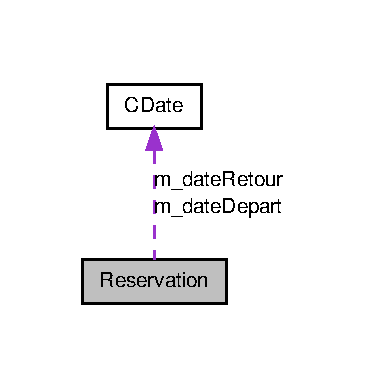
\includegraphics[width=176pt]{class_reservation__coll__graph}
\end{center}
\end{figure}
\subsection*{Fonctions membres publiques}
\begin{DoxyCompactItemize}
\item 
\hyperlink{class_reservation_ac7957aefcd95b0f9a36fa07f377a1072}{Reservation} (string veh, \hyperlink{class_c_date}{CDate} dateDep, \hyperlink{class_c_date}{CDate} dateRet)
\begin{DoxyCompactList}\small\item\em Constructeur. \item\end{DoxyCompactList}\item 
\hyperlink{class_reservation_a63b283053695e6f50fa44c50da2b3de5}{Reservation} ()
\begin{DoxyCompactList}\small\item\em Constructeur. \item\end{DoxyCompactList}\item 
\hyperlink{class_reservation_abf387b06b84f8a12c8e2e95d431d3d60}{$\sim$Reservation} ()
\begin{DoxyCompactList}\small\item\em Destructeur. \item\end{DoxyCompactList}\item 
void \hyperlink{class_reservation_ac72f95402ed4b92c2625ac8b546e95d0}{setDate} (char type, \hyperlink{class_c_date}{CDate} newDate)
\begin{DoxyCompactList}\small\item\em Modifier date. \item\end{DoxyCompactList}\item 
\hyperlink{class_c_date}{CDate} \hyperlink{class_reservation_ab03159e8f06b63e5dcd2f10ec637f1f8}{getDate} (char type)
\begin{DoxyCompactList}\small\item\em Obtenir date. \item\end{DoxyCompactList}\item 
void \hyperlink{class_reservation_a2760e98de6bd2b8c5259526962227a52}{afficher} (\hyperlink{class_parc}{Parc} p)
\begin{DoxyCompactList}\small\item\em Afficher resservation. \item\end{DoxyCompactList}\item 
void \hyperlink{class_reservation_af99771d51bffe33abf02c10ab67bbbc9}{save} (fstream \&outFile)
\begin{DoxyCompactList}\small\item\em Sauvegarder réservation. \item\end{DoxyCompactList}\item 
bool \hyperlink{class_reservation_a1d28645be56bc6d703786cc41fab5bdc}{estDisponible} (\hyperlink{class_c_date}{CDate} dep, \hyperlink{class_c_date}{CDate} ret)
\begin{DoxyCompactList}\small\item\em Vérifie disponibilité \item\end{DoxyCompactList}\item 
string \hyperlink{class_reservation_a987ccbdd8ba917b439e2282baaf5ea12}{getVehicule} ()
\begin{DoxyCompactList}\small\item\em Obtenir véhicule. \item\end{DoxyCompactList}\item 
bool \hyperlink{class_reservation_a5aa0fb5e7f6429bc414f02d4c7c5b142}{operator==} (\hyperlink{class_reservation}{Reservation} \&res) const 
\begin{DoxyCompactList}\small\item\em Réservations égales. \item\end{DoxyCompactList}\end{DoxyCompactItemize}


\subsection{Documentation des constructeurs et destructeur}
\hypertarget{class_reservation_ac7957aefcd95b0f9a36fa07f377a1072}{
\index{Reservation@{Reservation}!Reservation@{Reservation}}
\index{Reservation@{Reservation}!Reservation@{Reservation}}
\subsubsection[{Reservation}]{\setlength{\rightskip}{0pt plus 5cm}Reservation::Reservation (
\begin{DoxyParamCaption}
\item[{string}]{veh, }
\item[{{\bf CDate}}]{dateDep, }
\item[{{\bf CDate}}]{dateRet}
\end{DoxyParamCaption}
)}}
\label{class_reservation_ac7957aefcd95b0f9a36fa07f377a1072}


Constructeur. 

Constructeur de la classe \hyperlink{class_reservation}{Reservation}


\begin{DoxyParams}[1]{Paramètres}
\mbox{\tt in}  & {\em veh} & string, l'immatriculation du véhicule \\
\hline
\mbox{\tt in}  & {\em dateDep} & \hyperlink{class_c_date}{CDate}, la date de début de réservation \\
\hline
\mbox{\tt in}  & {\em dateRet} & \hyperlink{class_c_date}{CDate}, la date de fin de réservation \\
\hline
\end{DoxyParams}
\hypertarget{class_reservation_a63b283053695e6f50fa44c50da2b3de5}{
\index{Reservation@{Reservation}!Reservation@{Reservation}}
\index{Reservation@{Reservation}!Reservation@{Reservation}}
\subsubsection[{Reservation}]{\setlength{\rightskip}{0pt plus 5cm}Reservation::Reservation (
\begin{DoxyParamCaption}
{}
\end{DoxyParamCaption}
)}}
\label{class_reservation_a63b283053695e6f50fa44c50da2b3de5}


Constructeur. 

Constructeur par défaut de la classe \hyperlink{class_reservation}{Reservation}


\begin{DoxyParams}{Paramètres}
{\em aucun} & \\
\hline
\end{DoxyParams}
\hypertarget{class_reservation_abf387b06b84f8a12c8e2e95d431d3d60}{
\index{Reservation@{Reservation}!$\sim$Reservation@{$\sim$Reservation}}
\index{$\sim$Reservation@{$\sim$Reservation}!Reservation@{Reservation}}
\subsubsection[{$\sim$Reservation}]{\setlength{\rightskip}{0pt plus 5cm}Reservation::$\sim$Reservation (
\begin{DoxyParamCaption}
{}
\end{DoxyParamCaption}
)}}
\label{class_reservation_abf387b06b84f8a12c8e2e95d431d3d60}


Destructeur. 

Destructeur de la classe \hyperlink{class_reservation}{Reservation}


\begin{DoxyParams}{Paramètres}
{\em aucun} & \\
\hline
\end{DoxyParams}


\subsection{Documentation des fonctions membres}
\hypertarget{class_reservation_a2760e98de6bd2b8c5259526962227a52}{
\index{Reservation@{Reservation}!afficher@{afficher}}
\index{afficher@{afficher}!Reservation@{Reservation}}
\subsubsection[{afficher}]{\setlength{\rightskip}{0pt plus 5cm}void Reservation::afficher (
\begin{DoxyParamCaption}
\item[{{\bf Parc}}]{p}
\end{DoxyParamCaption}
)}}
\label{class_reservation_a2760e98de6bd2b8c5259526962227a52}


Afficher resservation. 

Affiche une réservation, en récupérant les caractéristiques du véhicule dans le parc passé en paramètre


\begin{DoxyParams}[1]{Paramètres}
\mbox{\tt in}  & {\em p} & \hyperlink{class_parc}{Parc}, le parc à explorer. Les informations sur les véhicules doivent être stockées dans une instance de la classe \hyperlink{class_parc}{Parc} \\
\hline
\end{DoxyParams}
\begin{DoxyReturn}{Renvoie}
void 
\end{DoxyReturn}
\hypertarget{class_reservation_a1d28645be56bc6d703786cc41fab5bdc}{
\index{Reservation@{Reservation}!estDisponible@{estDisponible}}
\index{estDisponible@{estDisponible}!Reservation@{Reservation}}
\subsubsection[{estDisponible}]{\setlength{\rightskip}{0pt plus 5cm}bool Reservation::estDisponible (
\begin{DoxyParamCaption}
\item[{{\bf CDate}}]{dep, }
\item[{{\bf CDate}}]{ret}
\end{DoxyParamCaption}
)}}
\label{class_reservation_a1d28645be56bc6d703786cc41fab5bdc}


Vérifie disponibilité 

Vérifie la disponibilité du véhicule dans la période comprise en deux dates


\begin{DoxyParams}[1]{Paramètres}
\mbox{\tt in}  & {\em dep} & \hyperlink{class_c_date}{CDate}, la date de départ souhaitée \\
\hline
\mbox{\tt in}  & {\em ret} & \hyperlink{class_c_date}{CDate}, la date de retour souhaitée \\
\hline
\end{DoxyParams}
\begin{DoxyReturn}{Renvoie}
bool vrai si le véhicule est disponible 

bool faux si le véhicule est indisponible 
\end{DoxyReturn}
\hypertarget{class_reservation_ab03159e8f06b63e5dcd2f10ec637f1f8}{
\index{Reservation@{Reservation}!getDate@{getDate}}
\index{getDate@{getDate}!Reservation@{Reservation}}
\subsubsection[{getDate}]{\setlength{\rightskip}{0pt plus 5cm}{\bf CDate} Reservation::getDate (
\begin{DoxyParamCaption}
\item[{char}]{type}
\end{DoxyParamCaption}
)}}
\label{class_reservation_ab03159e8f06b63e5dcd2f10ec637f1f8}


Obtenir date. 

Permet d'obtenir une date liée à une réservation


\begin{DoxyParams}[1]{Paramètres}
\mbox{\tt in}  & {\em type} & char, le type de date : d pour départ, r pour retour \\
\hline
\end{DoxyParams}
\begin{DoxyReturn}{Renvoie}
\hyperlink{class_c_date}{CDate} la date recherchée 
\end{DoxyReturn}
\hypertarget{class_reservation_a987ccbdd8ba917b439e2282baaf5ea12}{
\index{Reservation@{Reservation}!getVehicule@{getVehicule}}
\index{getVehicule@{getVehicule}!Reservation@{Reservation}}
\subsubsection[{getVehicule}]{\setlength{\rightskip}{0pt plus 5cm}string Reservation::getVehicule (
\begin{DoxyParamCaption}
{}
\end{DoxyParamCaption}
)}}
\label{class_reservation_a987ccbdd8ba917b439e2282baaf5ea12}


Obtenir véhicule. 

Renvoie le véhicule lié à la réservation


\begin{DoxyParams}{Paramètres}
{\em none} & \\
\hline
\end{DoxyParams}
\begin{DoxyReturn}{Renvoie}
string l'immatriculation du véhicule 
\end{DoxyReturn}
\hypertarget{class_reservation_a5aa0fb5e7f6429bc414f02d4c7c5b142}{
\index{Reservation@{Reservation}!operator==@{operator==}}
\index{operator==@{operator==}!Reservation@{Reservation}}
\subsubsection[{operator==}]{\setlength{\rightskip}{0pt plus 5cm}bool Reservation::operator== (
\begin{DoxyParamCaption}
\item[{{\bf Reservation} \&}]{res}
\end{DoxyParamCaption}
) const}}
\label{class_reservation_a5aa0fb5e7f6429bc414f02d4c7c5b142}


Réservations égales. 

Vérifie si deux réservations sont identiques


\begin{DoxyParams}[1]{Paramètres}
\mbox{\tt in,out}  & {\em res} & \hyperlink{class_reservation}{Reservation}, la réservation à comparer \\
\hline
\end{DoxyParams}
\begin{DoxyReturn}{Renvoie}
bool vrai si les deux réservations sont identiques (même véhicule et mêmes dates de départ et retour) 

bool faux si les deux réservations sont différentes. 
\end{DoxyReturn}
\hypertarget{class_reservation_af99771d51bffe33abf02c10ab67bbbc9}{
\index{Reservation@{Reservation}!save@{save}}
\index{save@{save}!Reservation@{Reservation}}
\subsubsection[{save}]{\setlength{\rightskip}{0pt plus 5cm}void Reservation::save (
\begin{DoxyParamCaption}
\item[{fstream \&}]{outFile}
\end{DoxyParamCaption}
)}}
\label{class_reservation_af99771d51bffe33abf02c10ab67bbbc9}


Sauvegarder réservation. 

Sauvegarde la réservation


\begin{DoxyParams}[1]{Paramètres}
\mbox{\tt in,out}  & {\em outFile} & fstream, le fichier de sauvegarde \\
\hline
\end{DoxyParams}
\begin{DoxyReturn}{Renvoie}
void 
\end{DoxyReturn}
\hypertarget{class_reservation_ac72f95402ed4b92c2625ac8b546e95d0}{
\index{Reservation@{Reservation}!setDate@{setDate}}
\index{setDate@{setDate}!Reservation@{Reservation}}
\subsubsection[{setDate}]{\setlength{\rightskip}{0pt plus 5cm}void Reservation::setDate (
\begin{DoxyParamCaption}
\item[{char}]{type, }
\item[{{\bf CDate}}]{newDate}
\end{DoxyParamCaption}
)}}
\label{class_reservation_ac72f95402ed4b92c2625ac8b546e95d0}


Modifier date. 

Permet de modifier les dates d'une réservation


\begin{DoxyParams}[1]{Paramètres}
\mbox{\tt in}  & {\em type} & char, le type de date : d pour départ, r pour retour \\
\hline
\mbox{\tt in}  & {\em newDate} & \hyperlink{class_c_date}{CDate}, la nouvelle date \\
\hline
\end{DoxyParams}
\begin{DoxyReturn}{Renvoie}
void 
\end{DoxyReturn}


La documentation de cette classe a été générée à partir du fichier suivant :\begin{DoxyCompactItemize}
\item 
inc/\hyperlink{_reservation_8h}{Reservation.h}\end{DoxyCompactItemize}

\hypertarget{class_tools}{
\section{Référence de la classe Tools}
\label{class_tools}\index{Tools@{Tools}}
}


Utilitaires.  




{\ttfamily \#include $<$Tools.h$>$}

\subsection*{Fonctions membres publiques statiques}
\begin{DoxyCompactItemize}
\item 
static int \hyperlink{class_tools_a1091376013e416681e90155ed87e977c}{isMinimum} (int a, int b)
\begin{DoxyCompactList}\small\item\em donne le minimum \item\end{DoxyCompactList}\item 
static bool \hyperlink{class_tools_a3b88f4e98469dd9d4cefcd0525aecde7}{estEntier} (const string \&data)
\begin{DoxyCompactList}\small\item\em Est entier. \item\end{DoxyCompactList}\item 
static bool \hyperlink{class_tools_ac293cf13e99e6d5739a5039cefa8753e}{estReel} (const string \&data)
\begin{DoxyCompactList}\small\item\em Est réel. \item\end{DoxyCompactList}\item 
static float \hyperlink{class_tools_a07892ec493ca75d5de5fbd01b1a7a223}{stringToFloat} (const string val)
\begin{DoxyCompactList}\small\item\em Conversion en réel. \item\end{DoxyCompactList}\item 
static void \hyperlink{class_tools_a53e25a53c9f01b0a7e5b3af7673d881d}{stringToLower} (string \&chaine)
\begin{DoxyCompactList}\small\item\em transforme en minuscules \item\end{DoxyCompactList}\item 
static void \hyperlink{class_tools_af1454104ca8edeb13cfbc7f6c39243d7}{stringToUpper} (string \&chaine)
\begin{DoxyCompactList}\small\item\em transforme en majuscules \item\end{DoxyCompactList}\item 
static void \hyperlink{class_tools_a19db87aec2d67f14d10bf8a3cc04ec02}{charToUpper} (char \&c)
\begin{DoxyCompactList}\small\item\em transforme en majuscules \item\end{DoxyCompactList}\item 
static void \hyperlink{class_tools_a0826e70408c956f4c4e481aeefe2d9e1}{charToLower} (char \&c)
\begin{DoxyCompactList}\small\item\em transforme en minuscules \item\end{DoxyCompactList}\item 
static int \hyperlink{class_tools_af0a210f513662ed4dffc8a79e39fa537}{stringToInt} (const string val)
\begin{DoxyCompactList}\small\item\em Conversion en entier. \item\end{DoxyCompactList}\end{DoxyCompactItemize}


\subsection{Description détaillée}
Utilitaires. Cette classe fournit un certain nombre de fonctions utilitaires, utilisables via des méthodes statiques.
\begin{DoxyItemize}
\item Conversion de chaînes de caractères en majuscules et minuscules
\item fonction de vérification et conversion d'entiers et réels depuis des chaînes de caractères 
\end{DoxyItemize}

\subsection{Documentation des fonctions membres}
\hypertarget{class_tools_a0826e70408c956f4c4e481aeefe2d9e1}{
\index{Tools@{Tools}!charToLower@{charToLower}}
\index{charToLower@{charToLower}!Tools@{Tools}}
\subsubsection[{charToLower}]{\setlength{\rightskip}{0pt plus 5cm}static void Tools::charToLower (
\begin{DoxyParamCaption}
\item[{char \&}]{c}
\end{DoxyParamCaption}
)\hspace{0.3cm}{\ttfamily  \mbox{[}static\mbox{]}}}}
\label{class_tools_a0826e70408c956f4c4e481aeefe2d9e1}


transforme en minuscules 

Transforme un caractère en lettre minuscule


\begin{DoxyParams}[1]{Paramètres}
\mbox{\tt in,out}  & {\em c,un} & caractères \\
\hline
\end{DoxyParams}
\begin{DoxyReturn}{Renvoie}
void 
\end{DoxyReturn}
\hypertarget{class_tools_a19db87aec2d67f14d10bf8a3cc04ec02}{
\index{Tools@{Tools}!charToUpper@{charToUpper}}
\index{charToUpper@{charToUpper}!Tools@{Tools}}
\subsubsection[{charToUpper}]{\setlength{\rightskip}{0pt plus 5cm}static void Tools::charToUpper (
\begin{DoxyParamCaption}
\item[{char \&}]{c}
\end{DoxyParamCaption}
)\hspace{0.3cm}{\ttfamily  \mbox{[}static\mbox{]}}}}
\label{class_tools_a19db87aec2d67f14d10bf8a3cc04ec02}


transforme en majuscules 

Transforme un caractère en lettre majuscule


\begin{DoxyParams}[1]{Paramètres}
\mbox{\tt in,out}  & {\em c,un} & caractère \\
\hline
\end{DoxyParams}
\begin{DoxyReturn}{Renvoie}
void 
\end{DoxyReturn}
\hypertarget{class_tools_a3b88f4e98469dd9d4cefcd0525aecde7}{
\index{Tools@{Tools}!estEntier@{estEntier}}
\index{estEntier@{estEntier}!Tools@{Tools}}
\subsubsection[{estEntier}]{\setlength{\rightskip}{0pt plus 5cm}static bool Tools::estEntier (
\begin{DoxyParamCaption}
\item[{const string \&}]{data}
\end{DoxyParamCaption}
)\hspace{0.3cm}{\ttfamily  \mbox{[}static\mbox{]}}}}
\label{class_tools_a3b88f4e98469dd9d4cefcd0525aecde7}


Est entier. 

Renvoie vrai si la chaîne de caractères fournie en paramètres est un entier


\begin{DoxyParams}[1]{Paramètres}
\mbox{\tt in,out}  & {\em data} & une chaîne de caractères \\
\hline
\end{DoxyParams}
\begin{DoxyReturn}{Renvoie}
vrai si data est un entier 

faux si data n'est pas un entier 
\end{DoxyReturn}
\hypertarget{class_tools_ac293cf13e99e6d5739a5039cefa8753e}{
\index{Tools@{Tools}!estReel@{estReel}}
\index{estReel@{estReel}!Tools@{Tools}}
\subsubsection[{estReel}]{\setlength{\rightskip}{0pt plus 5cm}static bool Tools::estReel (
\begin{DoxyParamCaption}
\item[{const string \&}]{data}
\end{DoxyParamCaption}
)\hspace{0.3cm}{\ttfamily  \mbox{[}static\mbox{]}}}}
\label{class_tools_ac293cf13e99e6d5739a5039cefa8753e}


Est réel. 

Renvoie vrai si la chaîne de caractères fournie en paramètres est un nombre réel


\begin{DoxyParams}[1]{Paramètres}
\mbox{\tt in,out}  & {\em data} & une chaîne de caractères \\
\hline
\end{DoxyParams}
\begin{DoxyReturn}{Renvoie}
vrai si data est un réel 

faux si data n'est pas un réel 
\end{DoxyReturn}
\hypertarget{class_tools_a1091376013e416681e90155ed87e977c}{
\index{Tools@{Tools}!isMinimum@{isMinimum}}
\index{isMinimum@{isMinimum}!Tools@{Tools}}
\subsubsection[{isMinimum}]{\setlength{\rightskip}{0pt plus 5cm}static int Tools::isMinimum (
\begin{DoxyParamCaption}
\item[{int}]{a, }
\item[{int}]{b}
\end{DoxyParamCaption}
)\hspace{0.3cm}{\ttfamily  \mbox{[}static\mbox{]}}}}
\label{class_tools_a1091376013e416681e90155ed87e977c}


donne le minimum 

Renvoie le plus petite valeur entre deux entiers fournis en paramètre


\begin{DoxyParams}[1]{Paramètres}
\mbox{\tt in}  & {\em a} & un entier \\
\hline
\mbox{\tt in}  & {\em b} & un entier \\
\hline
\end{DoxyParams}
\begin{DoxyReturn}{Renvoie}
entier, la valeur minimum entre a et b 
\end{DoxyReturn}
\hypertarget{class_tools_a07892ec493ca75d5de5fbd01b1a7a223}{
\index{Tools@{Tools}!stringToFloat@{stringToFloat}}
\index{stringToFloat@{stringToFloat}!Tools@{Tools}}
\subsubsection[{stringToFloat}]{\setlength{\rightskip}{0pt plus 5cm}static float Tools::stringToFloat (
\begin{DoxyParamCaption}
\item[{const string}]{val}
\end{DoxyParamCaption}
)\hspace{0.3cm}{\ttfamily  \mbox{[}static\mbox{]}}}}
\label{class_tools_a07892ec493ca75d5de5fbd01b1a7a223}


Conversion en réel. 

Convertit une chaine de caractères en nombre réel


\begin{DoxyParams}[1]{Paramètres}
\mbox{\tt in}  & {\em val} & une chaîne de caractères représentant un ,ombre réel \\
\hline
\end{DoxyParams}
\begin{DoxyReturn}{Renvoie}
float, un nombre réel 
\end{DoxyReturn}
\hypertarget{class_tools_af0a210f513662ed4dffc8a79e39fa537}{
\index{Tools@{Tools}!stringToInt@{stringToInt}}
\index{stringToInt@{stringToInt}!Tools@{Tools}}
\subsubsection[{stringToInt}]{\setlength{\rightskip}{0pt plus 5cm}static int Tools::stringToInt (
\begin{DoxyParamCaption}
\item[{const string}]{val}
\end{DoxyParamCaption}
)\hspace{0.3cm}{\ttfamily  \mbox{[}static\mbox{]}}}}
\label{class_tools_af0a210f513662ed4dffc8a79e39fa537}


Conversion en entier. 

Convertit une chaine de caractères en nombre entier


\begin{DoxyParams}[1]{Paramètres}
\mbox{\tt in}  & {\em val} & une chaîne de caractères représentant un entier \\
\hline
\end{DoxyParams}
\begin{DoxyReturn}{Renvoie}
int, un nombre réel 
\end{DoxyReturn}
\hypertarget{class_tools_a53e25a53c9f01b0a7e5b3af7673d881d}{
\index{Tools@{Tools}!stringToLower@{stringToLower}}
\index{stringToLower@{stringToLower}!Tools@{Tools}}
\subsubsection[{stringToLower}]{\setlength{\rightskip}{0pt plus 5cm}static void Tools::stringToLower (
\begin{DoxyParamCaption}
\item[{string \&}]{chaine}
\end{DoxyParamCaption}
)\hspace{0.3cm}{\ttfamily  \mbox{[}static\mbox{]}}}}
\label{class_tools_a53e25a53c9f01b0a7e5b3af7673d881d}


transforme en minuscules 

Transforme une chaîne de caractères en lettres minuscules


\begin{DoxyParams}[1]{Paramètres}
\mbox{\tt in,out}  & {\em chaine,une} & chaîne de caractères \\
\hline
\end{DoxyParams}
\begin{DoxyReturn}{Renvoie}
void 
\end{DoxyReturn}
\hypertarget{class_tools_af1454104ca8edeb13cfbc7f6c39243d7}{
\index{Tools@{Tools}!stringToUpper@{stringToUpper}}
\index{stringToUpper@{stringToUpper}!Tools@{Tools}}
\subsubsection[{stringToUpper}]{\setlength{\rightskip}{0pt plus 5cm}static void Tools::stringToUpper (
\begin{DoxyParamCaption}
\item[{string \&}]{chaine}
\end{DoxyParamCaption}
)\hspace{0.3cm}{\ttfamily  \mbox{[}static\mbox{]}}}}
\label{class_tools_af1454104ca8edeb13cfbc7f6c39243d7}


transforme en majuscules 

Transforme une chaîne de caractères en lettres majuscules


\begin{DoxyParams}[1]{Paramètres}
\mbox{\tt in,out}  & {\em chaine,une} & chaîne de caractères \\
\hline
\end{DoxyParams}
\begin{DoxyReturn}{Renvoie}
void 
\end{DoxyReturn}


La documentation de cette classe a été générée à partir du fichier suivant :\begin{DoxyCompactItemize}
\item 
inc/\hyperlink{_tools_8h}{Tools.h}\end{DoxyCompactItemize}

\hypertarget{class_utilitaire}{
\section{Référence de la classe Utilitaire}
\label{class_utilitaire}\index{Utilitaire@{Utilitaire}}
}


Graphe d'héritage de Utilitaire:
\nopagebreak
\begin{figure}[H]
\begin{center}
\leavevmode
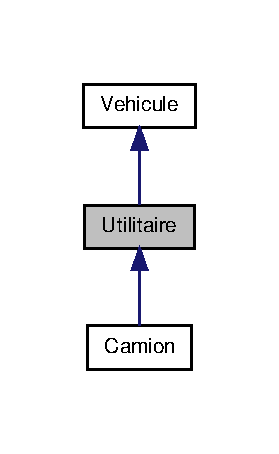
\includegraphics[width=134pt]{class_utilitaire__inherit__graph}
\end{center}
\end{figure}


Graphe de collaboration de Utilitaire:
\nopagebreak
\begin{figure}[H]
\begin{center}
\leavevmode
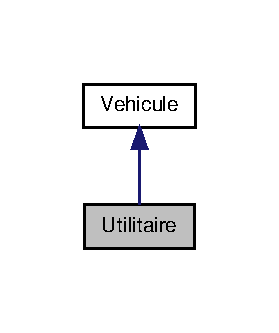
\includegraphics[width=134pt]{class_utilitaire__coll__graph}
\end{center}
\end{figure}
\subsection*{Fonctions membres publiques}
\begin{DoxyCompactItemize}
\item 
\hyperlink{class_utilitaire_a8fdab85b9894115b001e296eea151dec}{Utilitaire} (float volume, string immat, string marque, string modele)
\begin{DoxyCompactList}\small\item\em Constructeur. \item\end{DoxyCompactList}\item 
\hyperlink{class_utilitaire_a8a4af48b60aaeefe9b6399ed94495662}{Utilitaire} ()
\begin{DoxyCompactList}\small\item\em Constructeur. \item\end{DoxyCompactList}\item 
virtual \hyperlink{class_utilitaire_af6e70ea8eb994ab8744429b37d5a9934}{$\sim$Utilitaire} ()
\begin{DoxyCompactList}\small\item\em Destructeur. \item\end{DoxyCompactList}\item 
float \hyperlink{class_utilitaire_acde47d7bc100eb5fdf2195bb8307d36a}{getVolumeUtile} ()
\begin{DoxyCompactList}\small\item\em Récupérer volume utile. \item\end{DoxyCompactList}\item 
void \hyperlink{class_utilitaire_a085a6c510c036cbb88d91682751f3588}{setVolumeUtile} (float volume)
\begin{DoxyCompactList}\small\item\em Modifier volume utile. \item\end{DoxyCompactList}\item 
virtual void \hyperlink{class_utilitaire_a1092986e687a5a907bc86d252a8416c9}{afficher} ()
\begin{DoxyCompactList}\small\item\em Afficher utilitaire. \item\end{DoxyCompactList}\item 
virtual void \hyperlink{class_utilitaire_a7ee59be5d77191b06b2c959bdf2297b7}{save} (fstream \&fs)
\begin{DoxyCompactList}\small\item\em sauvegarder utilitaire \item\end{DoxyCompactList}\end{DoxyCompactItemize}


\subsection{Documentation des constructeurs et destructeur}
\hypertarget{class_utilitaire_a8fdab85b9894115b001e296eea151dec}{
\index{Utilitaire@{Utilitaire}!Utilitaire@{Utilitaire}}
\index{Utilitaire@{Utilitaire}!Utilitaire@{Utilitaire}}
\subsubsection[{Utilitaire}]{\setlength{\rightskip}{0pt plus 5cm}Utilitaire::Utilitaire (
\begin{DoxyParamCaption}
\item[{float}]{volume, }
\item[{string}]{immat, }
\item[{string}]{marque, }
\item[{string}]{modele}
\end{DoxyParamCaption}
)}}
\label{class_utilitaire_a8fdab85b9894115b001e296eea151dec}


Constructeur. 

Constructeur de la classe \hyperlink{class_vehicule}{Vehicule}


\begin{DoxyParams}[1]{Paramètres}
\mbox{\tt in}  & {\em volume} & réel, volume utile \\
\hline
\mbox{\tt in}  & {\em immat} & chaîne de caractères, le modèle du véhicule \\
\hline
\mbox{\tt in}  & {\em marque} & chaîne de caractères, la marque du véhicule \\
\hline
\mbox{\tt in}  & {\em modele} & chaîne de caractères, le kilométrage du véhicule \\
\hline
\end{DoxyParams}
\hypertarget{class_utilitaire_a8a4af48b60aaeefe9b6399ed94495662}{
\index{Utilitaire@{Utilitaire}!Utilitaire@{Utilitaire}}
\index{Utilitaire@{Utilitaire}!Utilitaire@{Utilitaire}}
\subsubsection[{Utilitaire}]{\setlength{\rightskip}{0pt plus 5cm}Utilitaire::Utilitaire (
\begin{DoxyParamCaption}
{}
\end{DoxyParamCaption}
)}}
\label{class_utilitaire_a8a4af48b60aaeefe9b6399ed94495662}


Constructeur. 

Constructeur par défaut de la classe \hyperlink{class_vehicule}{Vehicule} \hypertarget{class_utilitaire_af6e70ea8eb994ab8744429b37d5a9934}{
\index{Utilitaire@{Utilitaire}!$\sim$Utilitaire@{$\sim$Utilitaire}}
\index{$\sim$Utilitaire@{$\sim$Utilitaire}!Utilitaire@{Utilitaire}}
\subsubsection[{$\sim$Utilitaire}]{\setlength{\rightskip}{0pt plus 5cm}virtual Utilitaire::$\sim$Utilitaire (
\begin{DoxyParamCaption}
{}
\end{DoxyParamCaption}
)\hspace{0.3cm}{\ttfamily  \mbox{[}virtual\mbox{]}}}}
\label{class_utilitaire_af6e70ea8eb994ab8744429b37d5a9934}


Destructeur. 

Destructeur de la classe Ordre 

\subsection{Documentation des fonctions membres}
\hypertarget{class_utilitaire_a1092986e687a5a907bc86d252a8416c9}{
\index{Utilitaire@{Utilitaire}!afficher@{afficher}}
\index{afficher@{afficher}!Utilitaire@{Utilitaire}}
\subsubsection[{afficher}]{\setlength{\rightskip}{0pt plus 5cm}virtual void Utilitaire::afficher (
\begin{DoxyParamCaption}
{}
\end{DoxyParamCaption}
)\hspace{0.3cm}{\ttfamily  \mbox{[}virtual\mbox{]}}}}
\label{class_utilitaire_a1092986e687a5a907bc86d252a8416c9}


Afficher utilitaire. 

Affiche l'utilitaire


\begin{DoxyParams}{Paramètres}
{\em aucun} & \\
\hline
\end{DoxyParams}
\begin{DoxyReturn}{Renvoie}
void 
\end{DoxyReturn}


Réimplémentée à partir de \hyperlink{class_vehicule_aa83469d5e8e5fa9844cc52698b8ddf76}{Vehicule}.



Réimplémentée dans \hyperlink{class_camion_a1b7d9e844a03b1a1e7143a7618911157}{Camion}.

\hypertarget{class_utilitaire_acde47d7bc100eb5fdf2195bb8307d36a}{
\index{Utilitaire@{Utilitaire}!getVolumeUtile@{getVolumeUtile}}
\index{getVolumeUtile@{getVolumeUtile}!Utilitaire@{Utilitaire}}
\subsubsection[{getVolumeUtile}]{\setlength{\rightskip}{0pt plus 5cm}float Utilitaire::getVolumeUtile (
\begin{DoxyParamCaption}
{}
\end{DoxyParamCaption}
)}}
\label{class_utilitaire_acde47d7bc100eb5fdf2195bb8307d36a}


Récupérer volume utile. 

Renvoie le volume utile


\begin{DoxyParams}{Paramètres}
{\em none} & \\
\hline
\end{DoxyParams}
\begin{DoxyReturn}{Renvoie}
float le volume utile 
\end{DoxyReturn}
\hypertarget{class_utilitaire_a7ee59be5d77191b06b2c959bdf2297b7}{
\index{Utilitaire@{Utilitaire}!save@{save}}
\index{save@{save}!Utilitaire@{Utilitaire}}
\subsubsection[{save}]{\setlength{\rightskip}{0pt plus 5cm}virtual void Utilitaire::save (
\begin{DoxyParamCaption}
\item[{fstream \&}]{fs}
\end{DoxyParamCaption}
)\hspace{0.3cm}{\ttfamily  \mbox{[}virtual\mbox{]}}}}
\label{class_utilitaire_a7ee59be5d77191b06b2c959bdf2297b7}


sauvegarder utilitaire 

Sauvegarde l'utilitaire


\begin{DoxyParams}[1]{Paramètres}
\mbox{\tt in,out}  & {\em fs} & fstream, le fichier de sauvegarde \\
\hline
\end{DoxyParams}
\begin{DoxyReturn}{Renvoie}
void 
\end{DoxyReturn}


Réimplémentée à partir de \hyperlink{class_vehicule_a197353085208f6ceaf70c8e0303e4581}{Vehicule}.



Réimplémentée dans \hyperlink{class_camion_a2c715c85952a7e0bb2948494d79157b8}{Camion}.

\hypertarget{class_utilitaire_a085a6c510c036cbb88d91682751f3588}{
\index{Utilitaire@{Utilitaire}!setVolumeUtile@{setVolumeUtile}}
\index{setVolumeUtile@{setVolumeUtile}!Utilitaire@{Utilitaire}}
\subsubsection[{setVolumeUtile}]{\setlength{\rightskip}{0pt plus 5cm}void Utilitaire::setVolumeUtile (
\begin{DoxyParamCaption}
\item[{float}]{volume}
\end{DoxyParamCaption}
)}}
\label{class_utilitaire_a085a6c510c036cbb88d91682751f3588}


Modifier volume utile. 

Modifie le volume utile


\begin{DoxyParams}[1]{Paramètres}
\mbox{\tt in}  & {\em volume} & réel, le volume utile \\
\hline
\end{DoxyParams}
\begin{DoxyReturn}{Renvoie}
void 
\end{DoxyReturn}


La documentation de cette classe a été générée à partir du fichier suivant :\begin{DoxyCompactItemize}
\item 
inc/\hyperlink{_utilitaire_8h}{Utilitaire.h}\end{DoxyCompactItemize}

\hypertarget{class_vehicule}{
\section{Référence de la classe Vehicule}
\label{class_vehicule}\index{Vehicule@{Vehicule}}
}
Graphe d'héritage de Vehicule:\begin{figure}[H]
\begin{center}
\leavevmode
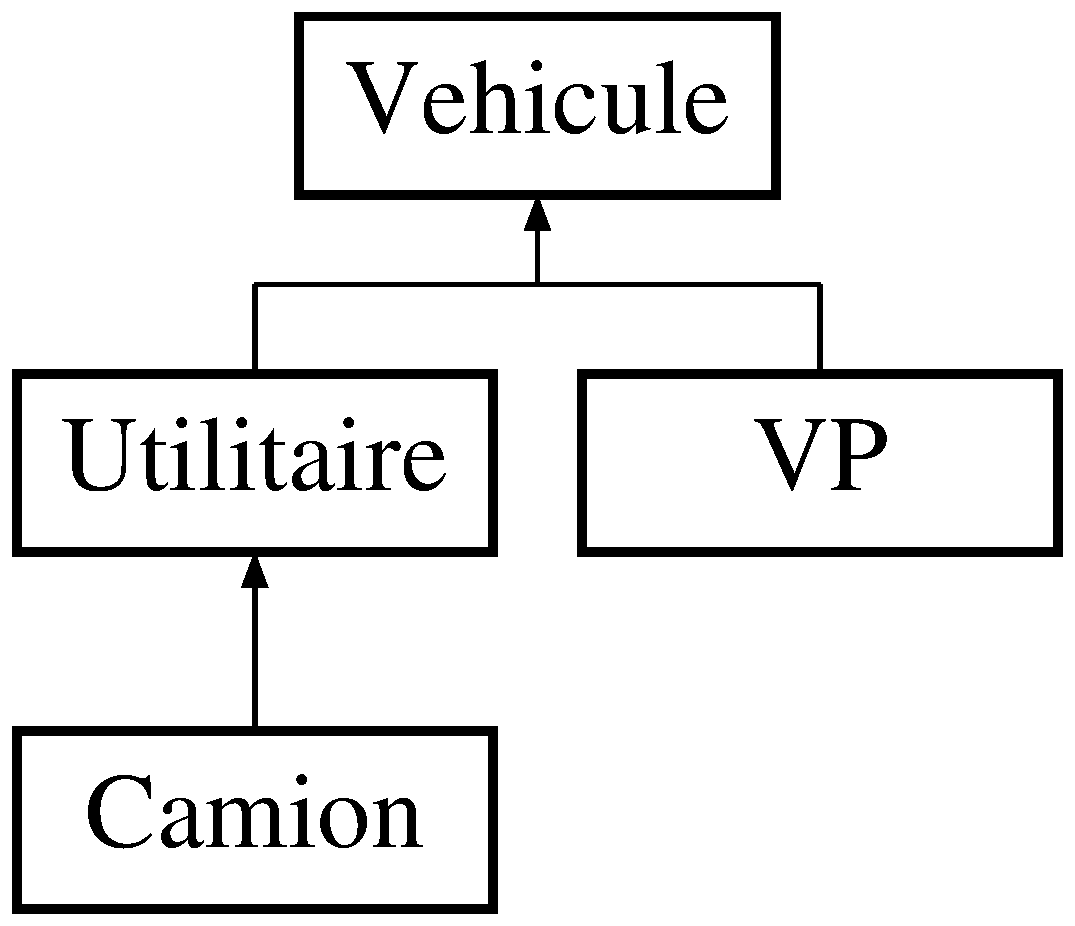
\includegraphics[height=3.000000cm]{class_vehicule}
\end{center}
\end{figure}
\subsection*{Fonctions membres publiques}
\begin{DoxyCompactItemize}
\item 
\hyperlink{class_vehicule_a860b5bc4192acc8061b79551e373df02}{Vehicule} (string immat, string marque, string modele, int kilometrage)
\begin{DoxyCompactList}\small\item\em Constructeur. \item\end{DoxyCompactList}\item 
\hyperlink{class_vehicule_ac9352572d0ca9cd4d3138247842c4ce8}{Vehicule} ()
\begin{DoxyCompactList}\small\item\em Constructeur. \item\end{DoxyCompactList}\item 
virtual \hyperlink{class_vehicule_af35800a1c217e3d39e91801932cc35ba}{$\sim$Vehicule} ()
\begin{DoxyCompactList}\small\item\em Destructeur. \item\end{DoxyCompactList}\item 
string \hyperlink{class_vehicule_a5be9ca3e75797e8009f1c9a8bd6f0f58}{getImmatriculation} ()
\begin{DoxyCompactList}\small\item\em Accéder immatriculation. \item\end{DoxyCompactList}\item 
void \hyperlink{class_vehicule_a8a70b407fbeb7cc7359d4c5cc4a11150}{setImmatriculation} (string immat)
\begin{DoxyCompactList}\small\item\em Modifier immatriculation. \item\end{DoxyCompactList}\item 
string \hyperlink{class_vehicule_a61fd72adc19ab2aaa08e3a36775f27ba}{getModele} ()
\begin{DoxyCompactList}\small\item\em Accéder modèle. \item\end{DoxyCompactList}\item 
void \hyperlink{class_vehicule_a877770a5a09ba45ec23c5d1befad2311}{setModele} (std::string modele)
\begin{DoxyCompactList}\small\item\em Modifier modele. \item\end{DoxyCompactList}\item 
string \hyperlink{class_vehicule_aca7733632f1a0f1f56d76726895a8c78}{getMarque} ()
\begin{DoxyCompactList}\small\item\em Accéder marque. \item\end{DoxyCompactList}\item 
void \hyperlink{class_vehicule_aa203aed9acca9590b347d119e14cf558}{setMarque} (std::string marque)
\begin{DoxyCompactList}\small\item\em Modifier marque. \item\end{DoxyCompactList}\item 
int \hyperlink{class_vehicule_ac5b3c0462bc23251f75da41208b6720c}{getKilometrage} ()
\begin{DoxyCompactList}\small\item\em Accéder kilométrage. \item\end{DoxyCompactList}\item 
void \hyperlink{class_vehicule_afe9c7d3740ae34ab098f1027a93329cd}{setKilometrage} (int kilom)
\begin{DoxyCompactList}\small\item\em Modifier kilométrage. \item\end{DoxyCompactList}\item 
bool \hyperlink{class_vehicule_afa55989329da4544093cad8e99b2f3b2}{operator==} (const \hyperlink{class_vehicule}{Vehicule} \&veh)
\begin{DoxyCompactList}\small\item\em Véhicule identiques. \item\end{DoxyCompactList}\item 
virtual void \hyperlink{class_vehicule_aa83469d5e8e5fa9844cc52698b8ddf76}{afficher} ()
\begin{DoxyCompactList}\small\item\em Afficher véhicule. \item\end{DoxyCompactList}\end{DoxyCompactItemize}


\subsection{Documentation des constructeurs et destructeur}
\hypertarget{class_vehicule_a860b5bc4192acc8061b79551e373df02}{
\index{Vehicule@{Vehicule}!Vehicule@{Vehicule}}
\index{Vehicule@{Vehicule}!Vehicule@{Vehicule}}
\subsubsection[{Vehicule}]{\setlength{\rightskip}{0pt plus 5cm}Vehicule::Vehicule (
\begin{DoxyParamCaption}
\item[{string}]{immat, }
\item[{string}]{marque, }
\item[{string}]{modele, }
\item[{int}]{kilometrage}
\end{DoxyParamCaption}
)}}
\label{class_vehicule_a860b5bc4192acc8061b79551e373df02}


Constructeur. 

Constructeur de la classe \hyperlink{class_vehicule}{Vehicule}


\begin{DoxyParams}{Paramètres}
{\em immat,chaîne} & de caractères, l'immatriculation du véhicule \\
\hline
{\em marque,chaîne} & de caractères, la marque du véhicule \\
\hline
{\em modele,chaîne} & de caractères, le modèle du véhicule \\
\hline
{\em kilometrage,entier,le} & kilométrage du véhicule \\
\hline
{\em nbLocation,entier,le} & nombre de locations du véhicule \\
\hline
\end{DoxyParams}
\hypertarget{class_vehicule_ac9352572d0ca9cd4d3138247842c4ce8}{
\index{Vehicule@{Vehicule}!Vehicule@{Vehicule}}
\index{Vehicule@{Vehicule}!Vehicule@{Vehicule}}
\subsubsection[{Vehicule}]{\setlength{\rightskip}{0pt plus 5cm}Vehicule::Vehicule (
\begin{DoxyParamCaption}
{}
\end{DoxyParamCaption}
)}}
\label{class_vehicule_ac9352572d0ca9cd4d3138247842c4ce8}


Constructeur. 

Constructeur par défaut de la classe \hyperlink{class_vehicule}{Vehicule}


\begin{DoxyParams}{Paramètres}
{\em aucun} & \\
\hline
\end{DoxyParams}
\hypertarget{class_vehicule_af35800a1c217e3d39e91801932cc35ba}{
\index{Vehicule@{Vehicule}!$\sim$Vehicule@{$\sim$Vehicule}}
\index{$\sim$Vehicule@{$\sim$Vehicule}!Vehicule@{Vehicule}}
\subsubsection[{$\sim$Vehicule}]{\setlength{\rightskip}{0pt plus 5cm}virtual Vehicule::$\sim$Vehicule (
\begin{DoxyParamCaption}
{}
\end{DoxyParamCaption}
)\hspace{0.3cm}{\ttfamily  \mbox{[}virtual\mbox{]}}}}
\label{class_vehicule_af35800a1c217e3d39e91801932cc35ba}


Destructeur. 

Destructeur de la classe \hyperlink{class_vehicule}{Vehicule}


\begin{DoxyParams}{Paramètres}
{\em aucun} & \\
\hline
\end{DoxyParams}


\subsection{Documentation des fonctions membres}
\hypertarget{class_vehicule_aa83469d5e8e5fa9844cc52698b8ddf76}{
\index{Vehicule@{Vehicule}!afficher@{afficher}}
\index{afficher@{afficher}!Vehicule@{Vehicule}}
\subsubsection[{afficher}]{\setlength{\rightskip}{0pt plus 5cm}virtual void Vehicule::afficher (
\begin{DoxyParamCaption}
{}
\end{DoxyParamCaption}
)\hspace{0.3cm}{\ttfamily  \mbox{[}virtual\mbox{]}}}}
\label{class_vehicule_aa83469d5e8e5fa9844cc52698b8ddf76}


Afficher véhicule. 

Affiche le véhicule


\begin{DoxyParams}{Paramètres}
{\em aucun} & \\
\hline
\end{DoxyParams}
\begin{DoxyReturn}{Renvoie}
void 
\end{DoxyReturn}


Réimplémentée dans \hyperlink{class_camion_a1b7d9e844a03b1a1e7143a7618911157}{Camion}, \hyperlink{class_utilitaire_a1092986e687a5a907bc86d252a8416c9}{Utilitaire}, et \hyperlink{class_v_p_a3af04349e81a3c643b497898ad19ef7a}{VP}.

\hypertarget{class_vehicule_a5be9ca3e75797e8009f1c9a8bd6f0f58}{
\index{Vehicule@{Vehicule}!getImmatriculation@{getImmatriculation}}
\index{getImmatriculation@{getImmatriculation}!Vehicule@{Vehicule}}
\subsubsection[{getImmatriculation}]{\setlength{\rightskip}{0pt plus 5cm}string Vehicule::getImmatriculation (
\begin{DoxyParamCaption}
{}
\end{DoxyParamCaption}
)}}
\label{class_vehicule_a5be9ca3e75797e8009f1c9a8bd6f0f58}


Accéder immatriculation. 

Permet d'obtenir l'immatriculation du véhicule


\begin{DoxyParams}{Paramètres}
{\em aucun} & \\
\hline
\end{DoxyParams}
\begin{DoxyReturn}{Renvoie}
m\_\-immatriculation, chaîne de caractères, l'immatriculation du véhicule 
\end{DoxyReturn}
\hypertarget{class_vehicule_ac5b3c0462bc23251f75da41208b6720c}{
\index{Vehicule@{Vehicule}!getKilometrage@{getKilometrage}}
\index{getKilometrage@{getKilometrage}!Vehicule@{Vehicule}}
\subsubsection[{getKilometrage}]{\setlength{\rightskip}{0pt plus 5cm}int Vehicule::getKilometrage (
\begin{DoxyParamCaption}
{}
\end{DoxyParamCaption}
)}}
\label{class_vehicule_ac5b3c0462bc23251f75da41208b6720c}


Accéder kilométrage. 

Permet d'obtenir le kilométrage du véhicule


\begin{DoxyParams}{Paramètres}
{\em aucun} & \\
\hline
\end{DoxyParams}
\begin{DoxyReturn}{Renvoie}
m\_\-kilometrage, entier, le kilométrage du véhicule 
\end{DoxyReturn}
\hypertarget{class_vehicule_aca7733632f1a0f1f56d76726895a8c78}{
\index{Vehicule@{Vehicule}!getMarque@{getMarque}}
\index{getMarque@{getMarque}!Vehicule@{Vehicule}}
\subsubsection[{getMarque}]{\setlength{\rightskip}{0pt plus 5cm}string Vehicule::getMarque (
\begin{DoxyParamCaption}
{}
\end{DoxyParamCaption}
)}}
\label{class_vehicule_aca7733632f1a0f1f56d76726895a8c78}


Accéder marque. 

Permet d'obtenir la marque du véhicule


\begin{DoxyParams}{Paramètres}
{\em aucun} & \\
\hline
\end{DoxyParams}
\begin{DoxyReturn}{Renvoie}
m\_\-marque, chaîne de caractères, la marque du véhicule 
\end{DoxyReturn}
\hypertarget{class_vehicule_a61fd72adc19ab2aaa08e3a36775f27ba}{
\index{Vehicule@{Vehicule}!getModele@{getModele}}
\index{getModele@{getModele}!Vehicule@{Vehicule}}
\subsubsection[{getModele}]{\setlength{\rightskip}{0pt plus 5cm}string Vehicule::getModele (
\begin{DoxyParamCaption}
{}
\end{DoxyParamCaption}
)}}
\label{class_vehicule_a61fd72adc19ab2aaa08e3a36775f27ba}


Accéder modèle. 

Permet d'obtenir le modèle du véhicule


\begin{DoxyParams}{Paramètres}
{\em aucun} & \\
\hline
\end{DoxyParams}
\begin{DoxyReturn}{Renvoie}
m\_\-modele, chaîne de caractères, le modèle du véhicule 
\end{DoxyReturn}
\hypertarget{class_vehicule_afa55989329da4544093cad8e99b2f3b2}{
\index{Vehicule@{Vehicule}!operator==@{operator==}}
\index{operator==@{operator==}!Vehicule@{Vehicule}}
\subsubsection[{operator==}]{\setlength{\rightskip}{0pt plus 5cm}bool Vehicule::operator== (
\begin{DoxyParamCaption}
\item[{const {\bf Vehicule} \&}]{veh}
\end{DoxyParamCaption}
)}}
\label{class_vehicule_afa55989329da4544093cad8e99b2f3b2}


Véhicule identiques. 

Permet de savoir si deux véhicules sont identiques


\begin{DoxyParams}{Paramètres}
{\em veh,objet} & \hyperlink{class_vehicule}{Vehicule}, le véhicule à comparer \\
\hline
\end{DoxyParams}
\begin{DoxyReturn}{Renvoie}
true s'il sont identiques 

false s'il sont différents 
\end{DoxyReturn}
\hypertarget{class_vehicule_a8a70b407fbeb7cc7359d4c5cc4a11150}{
\index{Vehicule@{Vehicule}!setImmatriculation@{setImmatriculation}}
\index{setImmatriculation@{setImmatriculation}!Vehicule@{Vehicule}}
\subsubsection[{setImmatriculation}]{\setlength{\rightskip}{0pt plus 5cm}void Vehicule::setImmatriculation (
\begin{DoxyParamCaption}
\item[{string}]{immat}
\end{DoxyParamCaption}
)}}
\label{class_vehicule_a8a70b407fbeb7cc7359d4c5cc4a11150}


Modifier immatriculation. 

Permet de modifier l'immatriculation du véhicule


\begin{DoxyParams}{Paramètres}
{\em immat,chaîne} & de caractères, l'immatriculation du véhicule \\
\hline
\end{DoxyParams}
\begin{DoxyReturn}{Renvoie}
void 
\end{DoxyReturn}
\hypertarget{class_vehicule_afe9c7d3740ae34ab098f1027a93329cd}{
\index{Vehicule@{Vehicule}!setKilometrage@{setKilometrage}}
\index{setKilometrage@{setKilometrage}!Vehicule@{Vehicule}}
\subsubsection[{setKilometrage}]{\setlength{\rightskip}{0pt plus 5cm}void Vehicule::setKilometrage (
\begin{DoxyParamCaption}
\item[{int}]{kilom}
\end{DoxyParamCaption}
)}}
\label{class_vehicule_afe9c7d3740ae34ab098f1027a93329cd}


Modifier kilométrage. 

Permet de modifier le kilométrage du véhicule


\begin{DoxyParams}{Paramètres}
{\em kilom,entier,le} & nouveau kilométrage du véhicule \\
\hline
\end{DoxyParams}
\begin{DoxyReturn}{Renvoie}
void 
\end{DoxyReturn}
\hypertarget{class_vehicule_aa203aed9acca9590b347d119e14cf558}{
\index{Vehicule@{Vehicule}!setMarque@{setMarque}}
\index{setMarque@{setMarque}!Vehicule@{Vehicule}}
\subsubsection[{setMarque}]{\setlength{\rightskip}{0pt plus 5cm}void Vehicule::setMarque (
\begin{DoxyParamCaption}
\item[{std::string}]{marque}
\end{DoxyParamCaption}
)}}
\label{class_vehicule_aa203aed9acca9590b347d119e14cf558}


Modifier marque. 

Permet de modifier la marque du véhicule


\begin{DoxyParams}{Paramètres}
{\em marque,chaîne} & de caractères, la marque du véhicule \\
\hline
\end{DoxyParams}
\begin{DoxyReturn}{Renvoie}
void 
\end{DoxyReturn}
\hypertarget{class_vehicule_a877770a5a09ba45ec23c5d1befad2311}{
\index{Vehicule@{Vehicule}!setModele@{setModele}}
\index{setModele@{setModele}!Vehicule@{Vehicule}}
\subsubsection[{setModele}]{\setlength{\rightskip}{0pt plus 5cm}void Vehicule::setModele (
\begin{DoxyParamCaption}
\item[{std::string}]{modele}
\end{DoxyParamCaption}
)}}
\label{class_vehicule_a877770a5a09ba45ec23c5d1befad2311}


Modifier modele. 

Permet de modifier le modèle du véhicule


\begin{DoxyParams}{Paramètres}
{\em modele,chaîne} & de caractères, le modèle du véhicule \\
\hline
\end{DoxyParams}
\begin{DoxyReturn}{Renvoie}
void 
\end{DoxyReturn}


La documentation de cette classe a été générée à partir du fichier suivant :\begin{DoxyCompactItemize}
\item 
inc/\hyperlink{_vehicule_8h}{Vehicule.h}\end{DoxyCompactItemize}

\hypertarget{class_v_p}{
\section{Référence de la classe VP}
\label{class_v_p}\index{VP@{VP}}
}


Graphe d'héritage de VP:
\nopagebreak
\begin{figure}[H]
\begin{center}
\leavevmode
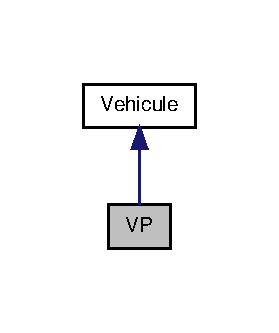
\includegraphics[width=134pt]{class_v_p__inherit__graph}
\end{center}
\end{figure}


Graphe de collaboration de VP:
\nopagebreak
\begin{figure}[H]
\begin{center}
\leavevmode
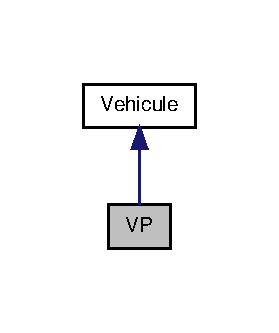
\includegraphics[width=134pt]{class_v_p__coll__graph}
\end{center}
\end{figure}
\subsection*{Fonctions membres publiques}
\begin{DoxyCompactItemize}
\item 
\hyperlink{class_v_p_a4bde97e27db770144037907d2eb0d081}{VP} (string immat, string marque, string modele, int nbPlaces)
\begin{DoxyCompactList}\small\item\em Constructeur. \item\end{DoxyCompactList}\item 
\hyperlink{class_v_p_ad67a48c8f2f8d3cc8466431d4e0c2949}{VP} ()
\begin{DoxyCompactList}\small\item\em Constructeur. \item\end{DoxyCompactList}\item 
virtual \hyperlink{class_v_p_ae9afa0cd76ea91730282e2ae82d0e203}{$\sim$VP} ()
\begin{DoxyCompactList}\small\item\em Destructeur. \item\end{DoxyCompactList}\item 
int \hyperlink{class_v_p_a6e6a4443cb9f83e0d94e3459b70bd73d}{getNbPlaces} ()
\begin{DoxyCompactList}\small\item\em Accéder nombre de places. \item\end{DoxyCompactList}\item 
void \hyperlink{class_v_p_a678d522ed1085e94814660d93edd9e7c}{setNbPlaces} (int nbPlaces)
\begin{DoxyCompactList}\small\item\em Modifier le nombre de places. \item\end{DoxyCompactList}\item 
virtual void \hyperlink{class_v_p_a3af04349e81a3c643b497898ad19ef7a}{afficher} ()
\begin{DoxyCompactList}\small\item\em Afficher \hyperlink{class_v_p}{VP}. \item\end{DoxyCompactList}\item 
virtual void \hyperlink{class_v_p_a3fe677e58cb952b7784d5f661ef426e6}{save} (fstream \&fs)
\begin{DoxyCompactList}\small\item\em sauvegarder \hyperlink{class_v_p}{VP} \item\end{DoxyCompactList}\end{DoxyCompactItemize}


\subsection{Documentation des constructeurs et destructeur}
\hypertarget{class_v_p_a4bde97e27db770144037907d2eb0d081}{
\index{VP@{VP}!VP@{VP}}
\index{VP@{VP}!VP@{VP}}
\subsubsection[{VP}]{\setlength{\rightskip}{0pt plus 5cm}VP::VP (
\begin{DoxyParamCaption}
\item[{string}]{immat, }
\item[{string}]{marque, }
\item[{string}]{modele, }
\item[{int}]{nbPlaces}
\end{DoxyParamCaption}
)}}
\label{class_v_p_a4bde97e27db770144037907d2eb0d081}


Constructeur. 

Constructeur de la classe \hyperlink{class_v_p}{VP}


\begin{DoxyParams}[1]{Paramètres}
\mbox{\tt in}  & {\em immat} & chaîne de caractères, l'immatriculation de la voiture \\
\hline
\mbox{\tt in}  & {\em modele} & chaîne de caractères, le modèle de la voiture \\
\hline
\mbox{\tt in}  & {\em marque} & chaîne de caractères, la marque de la voiture \\
\hline
\mbox{\tt in}  & {\em nbPlaces} & entier, le nombre de place de la voiture \\
\hline
\end{DoxyParams}
\hypertarget{class_v_p_ad67a48c8f2f8d3cc8466431d4e0c2949}{
\index{VP@{VP}!VP@{VP}}
\index{VP@{VP}!VP@{VP}}
\subsubsection[{VP}]{\setlength{\rightskip}{0pt plus 5cm}VP::VP (
\begin{DoxyParamCaption}
{}
\end{DoxyParamCaption}
)}}
\label{class_v_p_ad67a48c8f2f8d3cc8466431d4e0c2949}


Constructeur. 

Constructeur par défaut de la classe \hyperlink{class_v_p}{VP}


\begin{DoxyParams}{Paramètres}
{\em aucun} & \\
\hline
\end{DoxyParams}
\hypertarget{class_v_p_ae9afa0cd76ea91730282e2ae82d0e203}{
\index{VP@{VP}!$\sim$VP@{$\sim$VP}}
\index{$\sim$VP@{$\sim$VP}!VP@{VP}}
\subsubsection[{$\sim$VP}]{\setlength{\rightskip}{0pt plus 5cm}virtual VP::$\sim$VP (
\begin{DoxyParamCaption}
{}
\end{DoxyParamCaption}
)\hspace{0.3cm}{\ttfamily  \mbox{[}virtual\mbox{]}}}}
\label{class_v_p_ae9afa0cd76ea91730282e2ae82d0e203}


Destructeur. 

Destructeur de la classe \hyperlink{class_v_p}{VP}


\begin{DoxyParams}{Paramètres}
{\em aucun} & \\
\hline
\end{DoxyParams}


\subsection{Documentation des fonctions membres}
\hypertarget{class_v_p_a3af04349e81a3c643b497898ad19ef7a}{
\index{VP@{VP}!afficher@{afficher}}
\index{afficher@{afficher}!VP@{VP}}
\subsubsection[{afficher}]{\setlength{\rightskip}{0pt plus 5cm}virtual void VP::afficher (
\begin{DoxyParamCaption}
{}
\end{DoxyParamCaption}
)\hspace{0.3cm}{\ttfamily  \mbox{[}virtual\mbox{]}}}}
\label{class_v_p_a3af04349e81a3c643b497898ad19ef7a}


Afficher \hyperlink{class_v_p}{VP}. 

Affiche la voiture


\begin{DoxyParams}{Paramètres}
{\em aucun} & \\
\hline
\end{DoxyParams}
\begin{DoxyReturn}{Renvoie}
void 
\end{DoxyReturn}


Réimplémentée à partir de \hyperlink{class_vehicule_aa83469d5e8e5fa9844cc52698b8ddf76}{Vehicule}.

\hypertarget{class_v_p_a6e6a4443cb9f83e0d94e3459b70bd73d}{
\index{VP@{VP}!getNbPlaces@{getNbPlaces}}
\index{getNbPlaces@{getNbPlaces}!VP@{VP}}
\subsubsection[{getNbPlaces}]{\setlength{\rightskip}{0pt plus 5cm}int VP::getNbPlaces (
\begin{DoxyParamCaption}
{}
\end{DoxyParamCaption}
)}}
\label{class_v_p_a6e6a4443cb9f83e0d94e3459b70bd73d}


Accéder nombre de places. 

Permet d'obtenir le nombre de place de la voiture


\begin{DoxyParams}{Paramètres}
{\em aucun} & \\
\hline
\end{DoxyParams}
\begin{DoxyReturn}{Renvoie}
m\_\-nbPlaces entier, le nombre de place de la voiture 
\end{DoxyReturn}
\hypertarget{class_v_p_a3fe677e58cb952b7784d5f661ef426e6}{
\index{VP@{VP}!save@{save}}
\index{save@{save}!VP@{VP}}
\subsubsection[{save}]{\setlength{\rightskip}{0pt plus 5cm}virtual void VP::save (
\begin{DoxyParamCaption}
\item[{fstream \&}]{fs}
\end{DoxyParamCaption}
)\hspace{0.3cm}{\ttfamily  \mbox{[}virtual\mbox{]}}}}
\label{class_v_p_a3fe677e58cb952b7784d5f661ef426e6}


sauvegarder \hyperlink{class_v_p}{VP} 

Sauvegarde le \hyperlink{class_v_p}{VP}


\begin{DoxyParams}[1]{Paramètres}
\mbox{\tt in,out}  & {\em fs} & fstream, le fichier de sauvegarde \\
\hline
\end{DoxyParams}
\begin{DoxyReturn}{Renvoie}
void 
\end{DoxyReturn}


Réimplémentée à partir de \hyperlink{class_vehicule_a197353085208f6ceaf70c8e0303e4581}{Vehicule}.

\hypertarget{class_v_p_a678d522ed1085e94814660d93edd9e7c}{
\index{VP@{VP}!setNbPlaces@{setNbPlaces}}
\index{setNbPlaces@{setNbPlaces}!VP@{VP}}
\subsubsection[{setNbPlaces}]{\setlength{\rightskip}{0pt plus 5cm}void VP::setNbPlaces (
\begin{DoxyParamCaption}
\item[{int}]{nbPlaces}
\end{DoxyParamCaption}
)}}
\label{class_v_p_a678d522ed1085e94814660d93edd9e7c}


Modifier le nombre de places. 

Permet de modifier le nombre de place de la voiture


\begin{DoxyParams}[1]{Paramètres}
\mbox{\tt in}  & {\em nbPlaces} & entier, le nombre de place de la voiture \\
\hline
\end{DoxyParams}
\begin{DoxyReturn}{Renvoie}
void 
\end{DoxyReturn}


La documentation de cette classe a été générée à partir du fichier suivant :\begin{DoxyCompactItemize}
\item 
inc/\hyperlink{_v_p_8h}{VP.h}\end{DoxyCompactItemize}

\chapter{Documentation des fichiers}
\hypertarget{_camion_8h}{
\section{Référence du fichier inc/Camion.h}
\label{_camion_8h}\index{inc/Camion.h@{inc/Camion.h}}
}


Classe \hyperlink{class_camion}{Camion}.  


{\ttfamily \#include $<$iostream$>$}\par
{\ttfamily \#include $<$Utilitaire.h$>$}\par
\subsection*{Classes}
\begin{DoxyCompactItemize}
\item 
class \hyperlink{class_camion}{Camion}
\end{DoxyCompactItemize}


\subsection{Description détaillée}
Classe \hyperlink{class_camion}{Camion}. Cette classe permet de créer des camions, ie des utilitaires de plus de 3,5T. Pour les utilitaires de moins de 3,5t, il est conseillé d'utiliser la classe \hyperlink{class_utilitaire}{Utilitaire}

\begin{DoxyAuthor}{Auteur}
Gilles Coulais 
\end{DoxyAuthor}
\begin{DoxyVersion}{Version}
0.1 
\end{DoxyVersion}

\hypertarget{_c_date_8h}{
\section{Référence du fichier inc/CDate.h}
\label{_c_date_8h}\index{inc/CDate.h@{inc/CDate.h}}
}


Classe cdate.  


{\ttfamily \#include $<$string$>$}\par
{\ttfamily \#include $<$iostream$>$}\par
{\ttfamily \#include $<$time.h$>$}\par
{\ttfamily \#include $<$cstdlib$>$}\par
Graphe des dépendances par inclusion de CDate.h:
\nopagebreak
\begin{figure}[H]
\begin{center}
\leavevmode
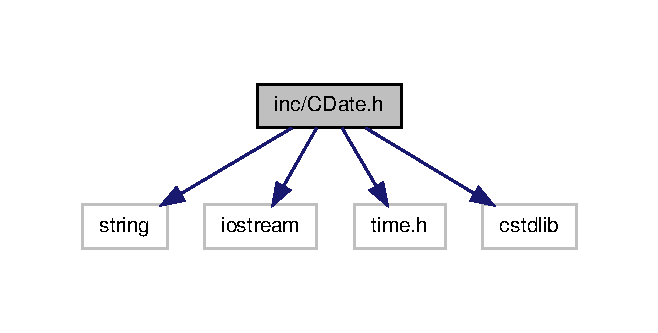
\includegraphics[width=316pt]{_c_date_8h__incl}
\end{center}
\end{figure}
Ce graphe montre quels fichiers incluent directement ou indirectement ce fichier :
\nopagebreak
\begin{figure}[H]
\begin{center}
\leavevmode
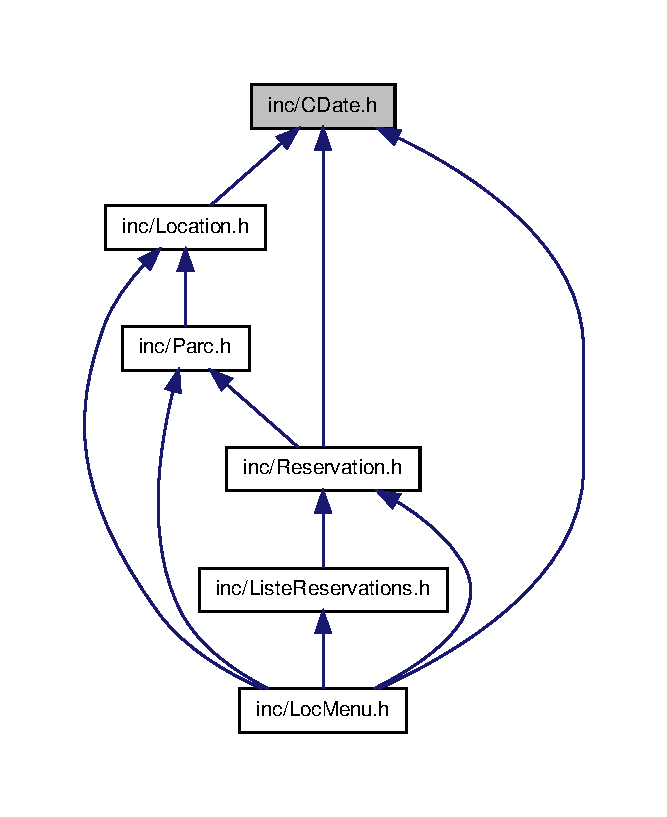
\includegraphics[width=320pt]{_c_date_8h__dep__incl}
\end{center}
\end{figure}
\subsection*{Classes}
\begin{DoxyCompactItemize}
\item 
class \hyperlink{class_c_date}{CDate}
\end{DoxyCompactItemize}


\subsection{Description détaillée}
Classe cdate. Cette classe propose des outils pour gérer une date

\begin{DoxyAuthor}{Auteur}
Franck Ruby, Gilles Coulais, Icham Sirat 
\end{DoxyAuthor}
\begin{DoxyVersion}{Version}
1.0 
\end{DoxyVersion}

\hypertarget{_liste_reservations_8h}{
\section{Référence du fichier inc/ListeReservations.h}
\label{_liste_reservations_8h}\index{inc/ListeReservations.h@{inc/ListeReservations.h}}
}


Classe \hyperlink{class_liste_reservations}{ListeReservations}.  


{\ttfamily \#include $<$iostream$>$}\par
{\ttfamily \#include $<$fstream$>$}\par
{\ttfamily \#include $<$list$>$}\par
{\ttfamily \#include $<$Reservation.h$>$}\par
Graphe des dépendances par inclusion de ListeReservations.h:\nopagebreak
\begin{figure}[H]
\begin{center}
\leavevmode
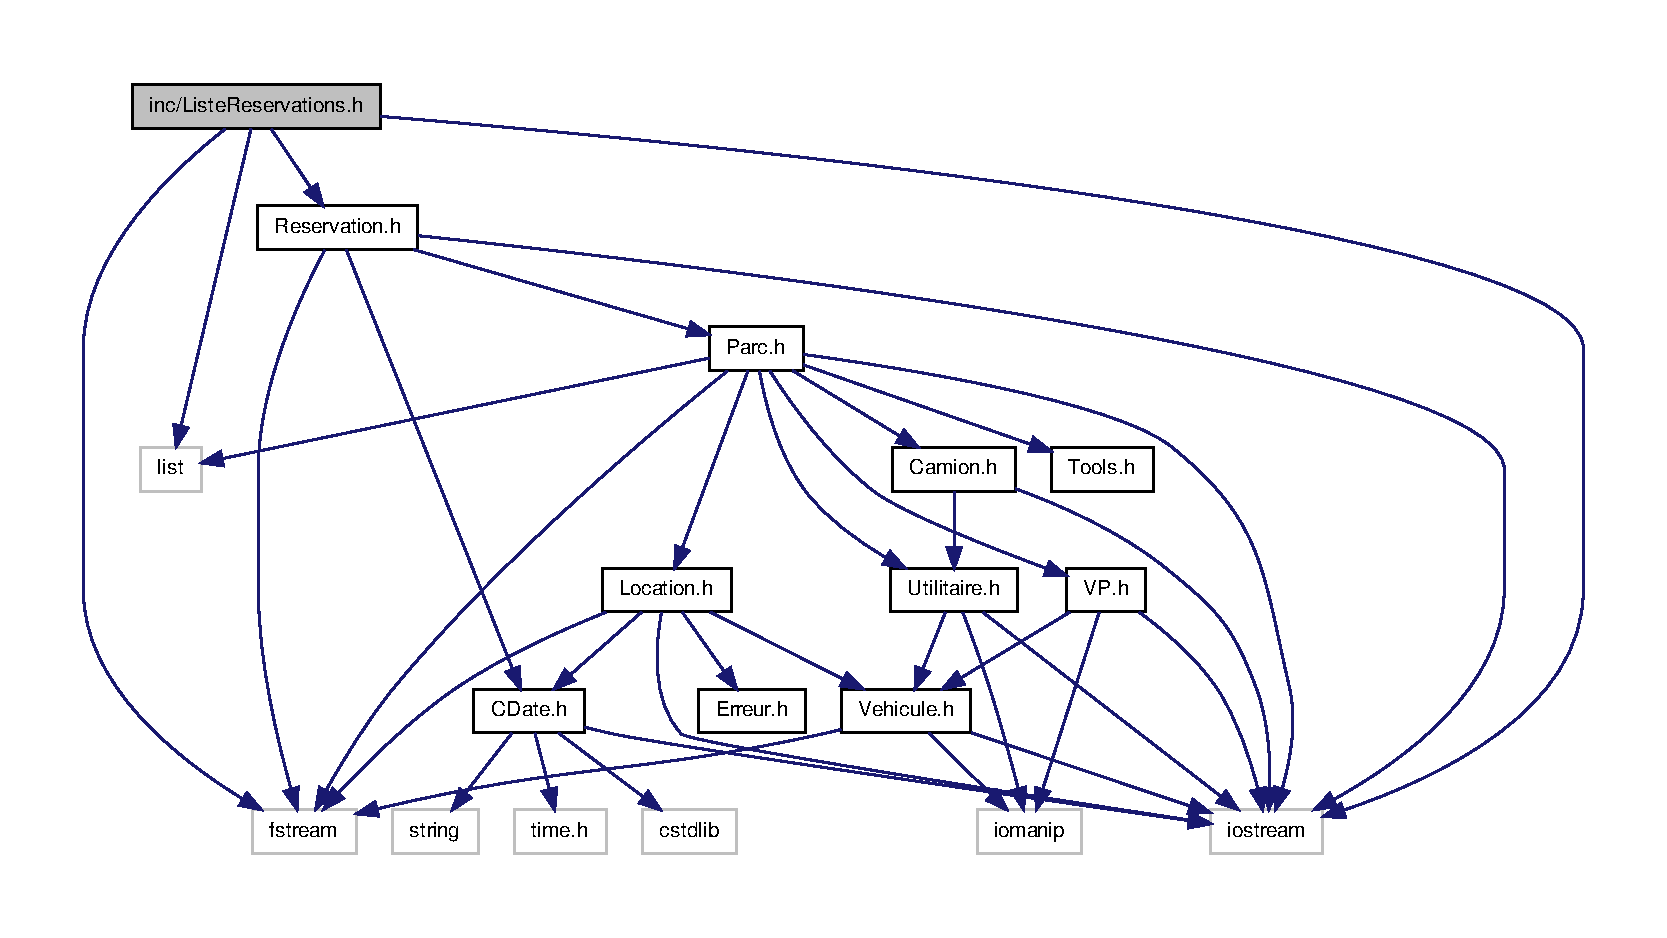
\includegraphics[width=400pt]{_liste_reservations_8h__incl}
\end{center}
\end{figure}
Ce graphe montre quels fichiers incluent directement ou indirectement ce fichier :\nopagebreak
\begin{figure}[H]
\begin{center}
\leavevmode
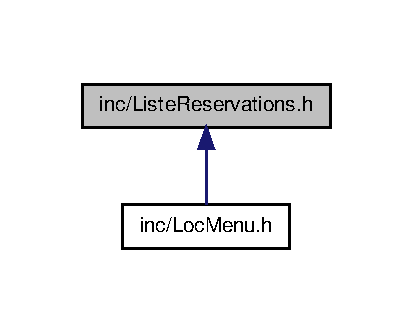
\includegraphics[width=198pt]{_liste_reservations_8h__dep__incl}
\end{center}
\end{figure}
\subsection*{Classes}
\begin{DoxyCompactItemize}
\item 
class \hyperlink{class_liste_reservations}{ListeReservations}
\begin{DoxyCompactList}\small\item\em Création de listes de réservations de véhicules. \item\end{DoxyCompactList}\end{DoxyCompactItemize}


\subsection{Description détaillée}
Classe \hyperlink{class_liste_reservations}{ListeReservations}. \begin{DoxyAuthor}{Auteur}
Gilles Coulais 
\end{DoxyAuthor}
\begin{DoxyVersion}{Version}
1.0 
\end{DoxyVersion}

\hypertarget{_location_8h}{
\section{Référence du fichier inc/Location.h}
\label{_location_8h}\index{inc/Location.h@{inc/Location.h}}
}


Classe \hyperlink{class_location}{Location}.  


{\ttfamily \#include $<$iostream$>$}\par
{\ttfamily \#include $<$fstream$>$}\par
{\ttfamily \#include $<$Vehicule.h$>$}\par
{\ttfamily \#include $<$CDate.h$>$}\par
{\ttfamily \#include $<$Erreur.h$>$}\par
Graphe des dépendances par inclusion de Location.h:\nopagebreak
\begin{figure}[H]
\begin{center}
\leavevmode
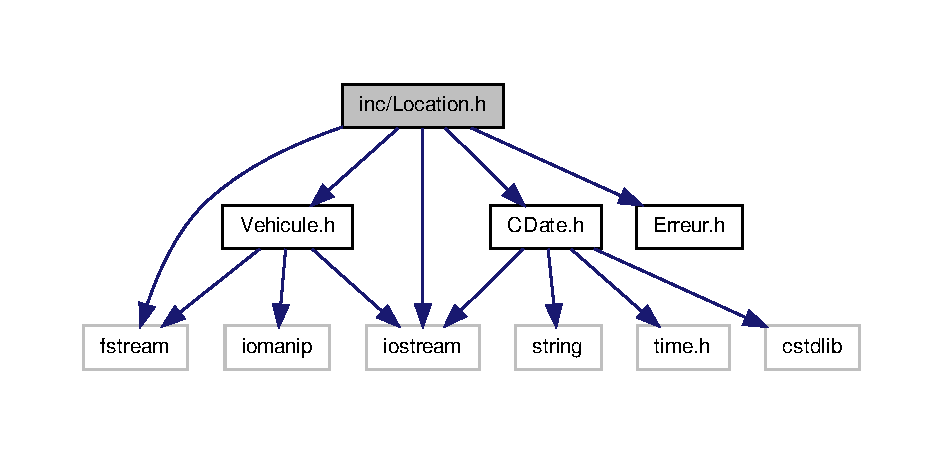
\includegraphics[width=400pt]{_location_8h__incl}
\end{center}
\end{figure}
Ce graphe montre quels fichiers incluent directement ou indirectement ce fichier :\nopagebreak
\begin{figure}[H]
\begin{center}
\leavevmode
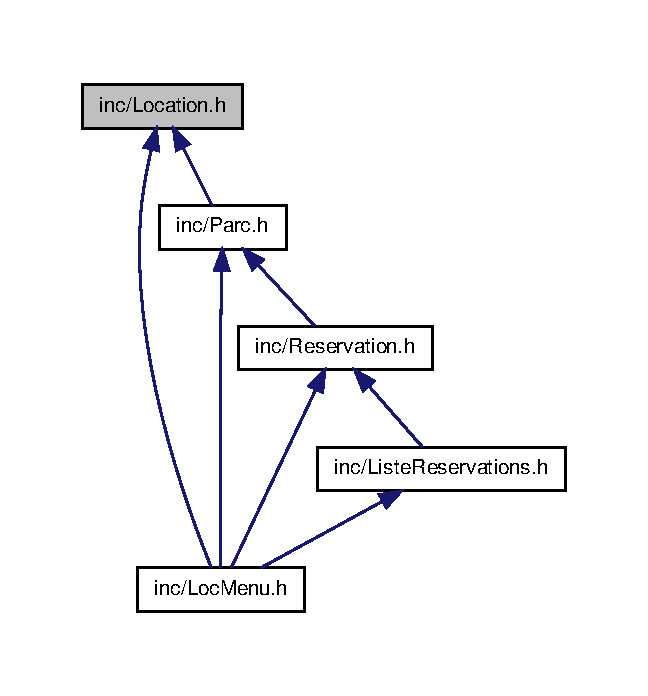
\includegraphics[width=311pt]{_location_8h__dep__incl}
\end{center}
\end{figure}
\subsection*{Classes}
\begin{DoxyCompactItemize}
\item 
class \hyperlink{class_location}{Location}
\end{DoxyCompactItemize}


\subsection{Description détaillée}
Classe \hyperlink{class_location}{Location}. Cette classe permet de gérer la location d'un véhicule

\begin{DoxyAuthor}{Auteur}
Gilles Coulais, Icham Sirat 
\end{DoxyAuthor}
\begin{DoxyVersion}{Version}
1.0 
\end{DoxyVersion}

\hypertarget{_loc_exception_8h}{
\section{Référence du fichier inc/LocException.h}
\label{_loc_exception_8h}\index{inc/LocException.h@{inc/LocException.h}}
}


Classe \hyperlink{class_loc_exception}{LocException}.  


{\ttfamily \#include $<$exception$>$}\par
{\ttfamily \#include $<$string$>$}\par
\subsection*{Classes}
\begin{DoxyCompactItemize}
\item 
class \hyperlink{class_loc_exception}{LocException}
\end{DoxyCompactItemize}


\subsection{Description détaillée}
Classe \hyperlink{class_loc_exception}{LocException}. Cette classe permet de gérer des exceptions. Elle dérive de la classe exception incluse dans la STL.

\begin{DoxyAuthor}{Auteur}
Icham Sirat 
\end{DoxyAuthor}
\begin{DoxyVersion}{Version}
0.1 
\end{DoxyVersion}

\hypertarget{_parc_8h}{
\section{Référence du fichier inc/Parc.h}
\label{_parc_8h}\index{inc/Parc.h@{inc/Parc.h}}
}


Classe \hyperlink{class_parc}{Parc}.  


{\ttfamily \#include $<$iostream$>$}\par
{\ttfamily \#include $<$fstream$>$}\par
{\ttfamily \#include $<$list$>$}\par
{\ttfamily \#include $<$Location.h$>$}\par
{\ttfamily \#include $<$Camion.h$>$}\par
{\ttfamily \#include $<$Utilitaire.h$>$}\par
{\ttfamily \#include $<$VP.h$>$}\par
{\ttfamily \#include $<$Tools.h$>$}\par
\subsection*{Classes}
\begin{DoxyCompactItemize}
\item 
class \hyperlink{class_parc}{Parc}
\end{DoxyCompactItemize}


\subsection{Description détaillée}
Classe \hyperlink{class_parc}{Parc}. Cette classe permet de gérer un parc de locations de véhicules

\begin{DoxyAuthor}{Auteur}
Gilles Coulais, Icham Sirat 
\end{DoxyAuthor}
\begin{DoxyVersion}{Version}
0.2 
\end{DoxyVersion}

\hypertarget{_reservation_8h}{
\section{Référence du fichier inc/Reservation.h}
\label{_reservation_8h}\index{inc/Reservation.h@{inc/Reservation.h}}
}


Classe \hyperlink{class_reservation}{Reservation}.  


{\ttfamily \#include $<$iostream$>$}\par
{\ttfamily \#include $<$fstream$>$}\par
{\ttfamily \#include $<$CDate.h$>$}\par
{\ttfamily \#include $<$Parc.h$>$}\par
\subsection*{Classes}
\begin{DoxyCompactItemize}
\item 
class \hyperlink{class_reservation}{Reservation}
\end{DoxyCompactItemize}


\subsection{Description détaillée}
Classe \hyperlink{class_reservation}{Reservation}. Cette classe permet de gérer une réservation de véhicule

\begin{DoxyAuthor}{Auteur}
Gilles Coulais 
\end{DoxyAuthor}
\begin{DoxyVersion}{Version}
0.1 
\end{DoxyVersion}

\hypertarget{_tools_8h}{
\section{Référence du fichier inc/Tools.h}
\label{_tools_8h}\index{inc/Tools.h@{inc/Tools.h}}
}


Utilitaires variés.  


\subsection*{Classes}
\begin{DoxyCompactItemize}
\item 
class \hyperlink{class_tools}{Tools}
\begin{DoxyCompactList}\small\item\em Utilitaires. \item\end{DoxyCompactList}\end{DoxyCompactItemize}


\subsection{Description détaillée}
Utilitaires variés. \begin{DoxyAuthor}{Auteur}
Gilles Coulais 
\end{DoxyAuthor}
\begin{DoxyVersion}{Version}
0.2 
\end{DoxyVersion}

\hypertarget{_utilitaire_8h}{
\section{Référence du fichier inc/Utilitaire.h}
\label{_utilitaire_8h}\index{inc/Utilitaire.h@{inc/Utilitaire.h}}
}


Classe \hyperlink{class_utilitaire}{Utilitaire}.  


{\ttfamily \#include $<$iostream$>$}\par
{\ttfamily \#include $<$iomanip$>$}\par
{\ttfamily \#include $<$Vehicule.h$>$}\par
Graphe des dépendances par inclusion de Utilitaire.h:
\nopagebreak
\begin{figure}[H]
\begin{center}
\leavevmode
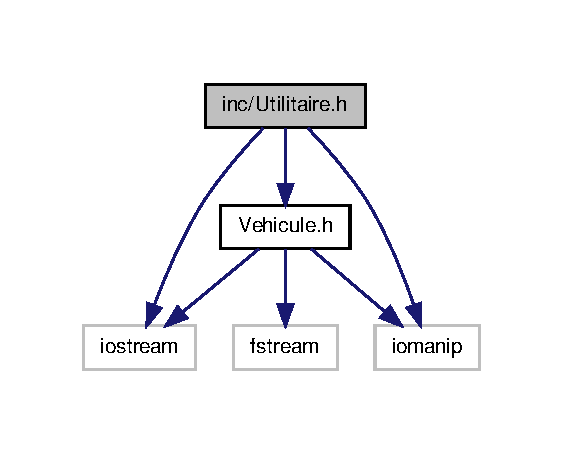
\includegraphics[width=270pt]{_utilitaire_8h__incl}
\end{center}
\end{figure}
Ce graphe montre quels fichiers incluent directement ou indirectement ce fichier :
\nopagebreak
\begin{figure}[H]
\begin{center}
\leavevmode
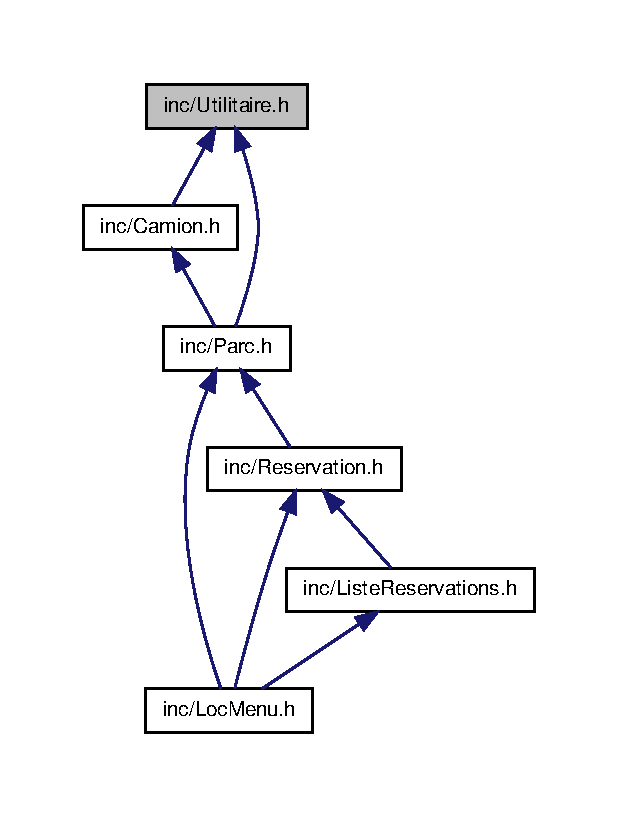
\includegraphics[width=296pt]{_utilitaire_8h__dep__incl}
\end{center}
\end{figure}
\subsection*{Classes}
\begin{DoxyCompactItemize}
\item 
class \hyperlink{class_utilitaire}{Utilitaire}
\end{DoxyCompactItemize}


\subsection{Description détaillée}
Classe \hyperlink{class_utilitaire}{Utilitaire}. Cette classe permet de créer des utilitaires. Pour les utilitaires de plus de 3,5t, il est conseillé d'utiliser la classe \hyperlink{class_camion}{Camion}

\begin{DoxyAuthor}{Auteur}
Gilles Coulais 
\end{DoxyAuthor}
\begin{DoxyVersion}{Version}
1.0 
\end{DoxyVersion}

\hypertarget{_vehicule_8h}{
\section{Référence du fichier inc/Vehicule.h}
\label{_vehicule_8h}\index{inc/Vehicule.h@{inc/Vehicule.h}}
}


Classe \hyperlink{class_vehicule}{Vehicule}.  


{\ttfamily \#include $<$iostream$>$}\par
{\ttfamily \#include $<$iomanip$>$}\par
\subsection*{Classes}
\begin{DoxyCompactItemize}
\item 
class \hyperlink{class_vehicule}{Vehicule}
\end{DoxyCompactItemize}


\subsection{Description détaillée}
Classe \hyperlink{class_vehicule}{Vehicule}. Cette classe propose un contenu basique pour créer un véhicule. Elle est destinée à être dérivée pour créer de nouvelles classes spécialisées.

\begin{DoxyAuthor}{Auteur}
Gilles Coulais, 

Icham Sirat 
\end{DoxyAuthor}
\begin{DoxyVersion}{Version}
0.2 
\end{DoxyVersion}

\hypertarget{_v_p_8h}{
\section{Référence du fichier inc/VP.h}
\label{_v_p_8h}\index{inc/VP.h@{inc/VP.h}}
}


Classe \hyperlink{class_v_p}{VP}.  


{\ttfamily \#include $<$iostream$>$}\par
{\ttfamily \#include $<$iomanip$>$}\par
{\ttfamily \#include $<$Vehicule.h$>$}\par
\subsection*{Classes}
\begin{DoxyCompactItemize}
\item 
class \hyperlink{class_v_p}{VP}
\end{DoxyCompactItemize}


\subsection{Description détaillée}
Classe \hyperlink{class_v_p}{VP}. Cette classe propose un contenu basique pour créer une voiture particulière.

\begin{DoxyAuthor}{Auteur}
Gilles Coulais, 

Icham Sirat 
\end{DoxyAuthor}
\begin{DoxyVersion}{Version}
0.2 
\end{DoxyVersion}

\printindex
\end{document}
